\documentclass[12pt,a4paper]{article}
\usepackage[a4paper, margin=0.8in, headheight=14pt]{geometry}
\usepackage{fontspec}
\usepackage{unicode-math}
\setmainfont{TeX Gyre Pagella}
\setmonofont[Scale=0.88]{TeX Gyre Cursor}
\setmathfont{Latin Modern Math}
\usepackage{xcolor}
\usepackage{colortbl}
\usepackage{titlesec}
\usepackage{enumitem}
\usepackage{tabularx}
\usepackage{booktabs}
\usepackage{array}
\usepackage{amsmath}
\usepackage{tikz}
\usetikzlibrary{shapes.geometric, arrows.meta, positioning, calc, fit, decorations.pathreplacing, decorations.pathmorphing}
\usepackage{tcolorbox}
\tcbuselibrary{skins, breakable}
\usepackage{hyperref}
\usepackage{fancyhdr}
\usepackage{graphicx}
\usepackage{microtype}
\hyphenpenalty=10000
\exhyphenpenalty=10000
\sloppy
\usepackage{caption}
\usepackage{setspace}
\usepackage{multirow}
\usepackage{tocloft}
\newcommand{\Q}[1]{\textbf{#1}\par\noindent\ignorespaces}
\definecolor{myred}{RGB}{196,30,58}
\definecolor{mydark}{RGB}{30,30,50}
\definecolor{mygreen}{RGB}{14,120,80}
\definecolor{myteal}{RGB}{0,130,140}
\definecolor{myamber}{RGB}{180,100,0}
\definecolor{mypurple}{RGB}{100,30,160}
\definecolor{mygray}{RGB}{246,247,249}
\definecolor{mgframe}{RGB}{180,185,200}
\definecolor{watermark}{RGB}{145,150,170}
\definecolor{hdrred}{RGB}{250,232,235}
\definecolor{hdrgreen}{RGB}{220,244,233}
\definecolor{hdrteal}{RGB}{220,242,244}
\definecolor{hdramber}{RGB}{253,242,215}
\definecolor{hdrpurple}{RGB}{238,228,255}
\definecolor{hdrgray}{RGB}{238,240,245}
\definecolor{rowalt}{RGB}{250,251,253}

\titleformat{\section}{\large\bfseries\color{myred}}{\thesection.}{0.5em}{}[\vspace{1pt}{\color{myred}\rule{\linewidth}{0.8pt}}]
\titleformat{\subsection}{\normalsize\bfseries\color{myteal}}{\thesubsection}{0.5em}{}
\titlespacing*{\section}{0pt}{18pt}{7pt}
\titlespacing*{\subsection}{0pt}{11pt}{4pt}
\setlength{\parindent}{0pt}
\setlength{\parskip}{4pt}
\renewcommand{\cfttoctitlefont}{\large\bfseries\color{myred}}
\renewcommand{\cftaftertoctitle}{\par\noindent{\color{myred}\rule{\linewidth}{0.8pt}}}
\setlength{\cftbeforetoctitleskip}{0pt}
\setlength{\cftaftertoctitleskip}{6pt}
\renewcommand{\cftsecfont}{\normalsize\bfseries\color{mydark}}
\renewcommand{\cftsecpagefont}{\normalsize\bfseries\color{mydark}}
\renewcommand{\cftsecleader}{\cftdotfill{\cftdotsep}}
\setlength{\cftbeforesecskip}{7pt}
\renewcommand{\cftsubsecfont}{\small\color{mydark}}
\renewcommand{\cftsubsecpagefont}{\small\color{mydark}}
\setlength{\cftbeforesubsecskip}{3pt}
\setlength{\cftsubsecindent}{1.4em}
\renewcommand{\cftpartfont}{\normalsize\bfseries\color{myteal}}
\renewcommand{\cftpartpagefont}{\normalsize\bfseries\color{myteal}}
\setlength{\cftbeforepartskip}{14pt}
\renewcommand{\arraystretch}{1.45}
\setlength{\tabcolsep}{6pt}
\arrayrulecolor{mydark}
\newcolumntype{B}[1]{>{\small\bfseries\raggedright\arraybackslash}m{#1}}
\newcolumntype{C}[1]{>{\centering\arraybackslash}m{#1}}
\newcolumntype{Y}{>{\small\raggedright\arraybackslash}X}
\renewcommand{\tabularxcolumn}[1]{m{#1}}
\newcommand{\currmodule}{Module 1}
\pagestyle{fancy}
\fancyhf{}
\fancyhead[L]{\small\color{myred}\textbf{PE-EC702B}\;\color{mydark}--- Digital Image and Video Processing}
\fancyhead[R]{\small\color{myteal}\textbf{\currmodule\ Notes}}
\fancyfoot[C]{\small\color{mydark}\thepage}
\fancyfoot[R]{\small\color{watermark}\textit{\copyright\ Biraj}}
\renewcommand{\headrulewidth}{0.5pt}
\renewcommand{\footrulewidth}{0.3pt}

\hypersetup{colorlinks=true, linkcolor=myteal, urlcolor=myteal,
  pdfauthor={Biraj Sarkar},
  pdftitle={PE-EC702B --- Combined Notes}}

\tcbset{
  tikzbox/.style={
    colback=mygray, colframe=mgframe, boxrule=0.6pt, arc=4pt,
    left=8pt, right=8pt, top=6pt, bottom=6pt,
    colbacktitle=mgframe, coltitle=mydark,
    fonttitle=\small\bfseries
  },
  defbox/.style={
    colback=hdrgreen, colframe=mygreen, boxrule=0.8pt, arc=4pt,
    left=9pt, right=9pt, top=6pt, bottom=6pt,
    colbacktitle=mygreen, coltitle=white,
    fonttitle=\small\bfseries
  },
  formulabox/.style={
    colback=hdrteal, colframe=myteal, boxrule=0.8pt, arc=4pt,
    left=9pt, right=9pt, top=7pt, bottom=7pt,
    colbacktitle=myteal, coltitle=white,
    fonttitle=\small\bfseries
  },
  examplebox/.style={
    colback=hdramber, colframe=myamber, boxrule=0.8pt, arc=4pt,
    left=9pt, right=9pt, top=6pt, bottom=6pt,
    colbacktitle=myamber, coltitle=white,
    fonttitle=\small\bfseries,
    breakable
  },
  masonbox/.style={
    colback=hdrpurple, colframe=mypurple, boxrule=0.8pt, arc=4pt,
    left=9pt, right=9pt, top=6pt, bottom=6pt,
    colbacktitle=mypurple, coltitle=white,
    fonttitle=\small\bfseries
  },
  exambox/.style={
    colback=hdrpurple, colframe=mypurple, boxrule=1pt, arc=5pt,
    left=10pt, right=10pt, top=8pt, bottom=8pt,
    colbacktitle=mypurple, coltitle=white,
    fonttitle=\bfseries,
    breakable, title after break={\textbf{Frequently Asked / Viva Questions (contd.)}}}
}
\tcbset{after={\color{black}}}

\tikzset{
  block/.style={rectangle, draw=myteal, fill=hdrteal,
    text width=2.2cm, align=center, minimum height=0.85cm,
    font=\small, rounded corners=3pt, line width=0.7pt},
  arrow/.style={-Stealth, thick, color=mydark},
  redarrow/.style={-Stealth, thick, color=myred},
  line/.style={thick, color=mydark}
}

\newcommand{\modulestart}[2]{%
  \clearpage
  \renewcommand{\currmodule}{Module #1}%
  \phantomsection
  \addcontentsline{toc}{part}{Module #1: #2}%
  \setcounter{section}{0}%
  \begin{center}
    \vspace*{1.0cm}
    {\Huge\bfseries\color{myred} Module #1}\\[10pt]
    {\Large\bfseries\color{mydark} #2}\\[10pt]
    {\color{myred}\rule{0.55\linewidth}{1.2pt}}
  \end{center}
  \vspace{14pt}
}
\begin{document}

\thispagestyle{empty}
\vspace*{1.0cm}
\begin{center}
  {\Huge\bfseries\color{myred} PE-EC702B}\\[10pt]
  {\LARGE\bfseries\color{mydark} Digital Image and Video Processing}\\[20pt]
  {\color{myred}\rule{0.7\linewidth}{1.5pt}}\\[18pt]
  {\Large\color{myteal}\textbf{Combined Module Notes}}\\[8pt]
  {\large\color{mydark} Modules 1 -- 8}\\[40pt]
  {\normalsize\color{mydark} Semester VII \quad$\bullet$\quad 3L:0T:0P \quad$\bullet$\quad 3 Credits}\\[12pt]
  {\normalsize\color{mydark} CGEC \;$|$\; B.Tech ECE (2023--27)}\\[6pt]
  {\normalsize\color{mydark}\textit{Biraj Sarkar}}
\end{center}
\vspace{1.0cm}
\begin{center}
  \begin{tcolorbox}[colback=mygray, colframe=mgframe, boxrule=0.5pt, arc=3pt, width=0.85\linewidth]
    \centering\small\color{mydark}
    \textbf{Disclaimer / Study Guide Notice:}\\
    These are condensed \textbf{Short Notes} focusing on core theory, key formulas, block/circuit diagrams, and standard viva Q\&As for university exam revision. Exhaustive numerical practice problems and derivation edge cases are not covered. This serves as a quick-revision reference guide for students.
  \end{tcolorbox}
\end{center}
\vfill
\begin{center}{\small\color{watermark}\textit{Exam-Ready Notes}}\end{center}
\clearpage

\hypersetup{linkcolor=mydark}
\tableofcontents
\hypersetup{linkcolor=myteal}
\clearpage

% -- Module 1 -----------------------------------------------------------------
\modulestart{1}{Elements of Visual Perception}

\section{Elements of Visual Perception}
% ===============================================================================

Understanding human visual perception is crucial for digital image processing because the human eye is the ultimate receiver of the visual output.

\begin{tcolorbox}[defbox, title={Visual Perception Fundamentals}]
\textbf{Brightness Adaptation:} The human eye can operate over an enormous dynamic range ($10^{10}$ units), but cannot view this entire range simultaneously. It accomplishes this by changing its overall sensitivity, a process known as \textit{brightness adaptation}.
\end{tcolorbox}

\subsection{Eye Structure and Receptors}
The human eye contains two primary photoreceptors located on the retina:
\begin{itemize}[leftmargin=*, itemsep=2.5pt]
  \item \textbf{Cones (Photopic Vision):} Approximately 6 to 7 million receptors located mainly in the central portion of the retina (fovea). Highly sensitive to color. Allows resolve of fine details.
  \item \textbf{Rods (Scotopic Vision):} Approximately 75 to 150 million receptors distributed over the retinal surface. Give a general, overall picture of the field of view. Sensitive to low illumination levels (night vision), but are color-blind.
\end{itemize}

\subsection{Contrast Discrimination and Weber Ratio}
The ability of the eye to discriminate between different intensity levels is characterized by the \textbf{Weber Ratio}.
\begin{itemize}[leftmargin=*, itemsep=3pt]
  \item A subject is exposed to a uniform background intensity $I$.
  \item A short duration increment $\Delta I$ is added.
  \item The ratio $\frac{\Delta I}{I}$ at which the subject can just detect the change is called the \textbf{Weber Fraction}.
  \item A small Weber fraction indicates good intensity discrimination (high sensitivity), whereas a large fraction indicates poor discrimination (occurring at low illumination).
\end{itemize}

% ===============================================================================
\section{Image Sensing and Acquisition}
% ===============================================================================

To generate a digital image, the physical energy (light, X-ray, electromagnetic wave) must be converted into electrical signals by sensors.

\begin{tcolorbox}[defbox, title={Image Sensor Configurations}]
\textbf{Image Sensors:} Devices that convert illumination energy into electrical voltage. There are three primary configurations:
\begin{enumerate}[label=(\alph*), leftmargin=*, itemsep=1pt]
  \item \textbf{Single Sensor:} Uses a photodiode that moves mechanically in $x$- and $y$-directions (e.g., microdensitometers).
  \item \textbf{Sensor Strips:} Inline array of sensors providing 1D line scans (e.g., flatbed scanners).
  \item \textbf{Sensor Array:} 2D grid of sensors capturing the entire scene (e.g., CCD/CMOS arrays in digital cameras).
\end{enumerate}
\end{tcolorbox}

% ===============================================================================
\section{Image Sampling and Quantization}
% ===============================================================================

A continuous image $f(x,y)$ must be converted into digital format in both spatial coordinates (sampling) and amplitude (quantization).

\begin{tcolorbox}[defbox, title={Sampling vs. Quantization}]
\textbf{Sampling:} Digitizing the continuous spatial coordinates $(x,y)$ into discrete grid indices.
\par\noindent
\textbf{Quantization:} Digitizing the continuous amplitude (intensity values) into discrete gray levels.
\end{tcolorbox}

\subsection{Representing Digital Images}
A digital image of size $M \times N$ with $L$ discrete gray levels is represented as a matrix:
\begin{equation}
  f(x,y) = \begin{bmatrix}
    f(0,0) & f(0,1) & \cdots & f(0,N-1) \\
    f(1,0) & f(1,1) & \cdots & f(1,N-1) \\
    \vdots & \vdots & \ddots & \vdots \\
    f(M-1,0) & f(M-1,1) & \cdots & f(M-1,N-1)
  \end{bmatrix}
\end{equation}
The number of gray levels $L$ is typically a power of 2:
\begin{equation}
  L = 2^k
\end{equation}
where $k$ is the number of bits required to store each pixel. The total number of bits $b$ required to store the image is:
\begin{equation}
  b = M \times N \times k
\end{equation}

\subsection{Resolution and Spatial Regressions}
\begin{itemize}[leftmargin=*, itemsep=3.5pt]
  \item \textbf{Spatial Resolution:} The smallest discernible detail in an image, measured in dots/pixels per unit distance (e.g., dpi). Insufficient spatial sampling causes \textbf{aliasing} (moir\'{e} patterns).
  \item \textbf{Intensity Resolution:} The smallest discernible change in gray level, measured in bits per pixel.
  \item \textbf{False Contouring:} An effect caused by insufficient quantization levels (typically $k < 4$ bits), producing visible, artificial boundaries between smooth gray-level transitions.
\end{itemize}

% ===============================================================================
\section{Basic Relationships Between Pixels}
% ===============================================================================

Let $p$ and $q$ be pixels in an image. Their relationships determine boundaries, regions, and structures.

\subsection{Pixel Neighborhoods}
\begin{itemize}[leftmargin=*, itemsep=3.5pt]
  \item \textbf{4-neighbors ($N_4(p)$):} The 4 horizontal and vertical pixels adjacent to $p$ at coordinates:
    \begin{equation}
      (x+1, y), \quad (x-1, y), \quad (x, y+1), \quad (x, y-1)
    \end{equation}
  \item \textbf{Diagonal neighbors ($N_D(p)$):} The 4 diagonal pixels adjacent to $p$ at coordinates:
    \begin{equation}
      (x+1, y+1), \quad (x+1, y-1), \quad (x-1, y+1), \quad (x-1, y-1)
    \end{equation}
  \item \textbf{8-neighbors ($N_8(p)$):} The union of 4-neighbors and diagonal neighbors:
    \begin{equation}
      N_8(p) = N_4(p) \cup N_D(p)
    \end{equation}
\end{itemize}

\subsection{Adjacency and Path Connectivity}
Let $V$ be the set of intensity values used to define adjacency (e.g., $V = \{1\}$ in binary images, or $V = \{128, \dots, 255\}$ in grayscale).
\begin{enumerate}[leftmargin=*, itemsep=3.5pt]
  \item \textbf{4-adjacency:} Two pixels $p$ and $q$ with values in $V$ are 4-adjacent if $q \in N_4(p)$.
  \item \textbf{8-adjacency:} Two pixels $p$ and $q$ with values in $V$ are 8-adjacent if $q \in N_8(p)$.
  \item \textbf{m-adjacency (mixed adjacency):} Two pixels $p$ and $q$ with values in $V$ are m-adjacent if:
    \begin{itemize}[leftmargin=1.5em, itemsep=1pt]
      \item $q \in N_4(p)$, OR
      \item $q \in N_D(p)$ and the intersection $N_4(p) \cap N_4(q)$ has no pixels with values from $V$.
    \end{itemize}
    \textit{Purpose: m-adjacency is introduced to eliminate the multiple path ambiguities that arise in 8-adjacency.}
\end{enumerate}

\begin{tcolorbox}[tikzbox, title={Pixel Neighborhoods and m-Adjacency}]
\centering
\begin{minipage}{0.45\textwidth}
  \centering
  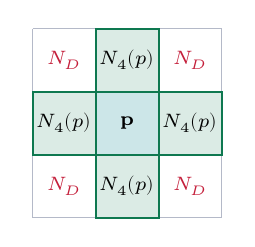
\begin{tikzpicture}[scale=0.8, every node/.style={font=\scriptsize}]
    % Neighbor Grid
    \draw[step=1.0cm, color=mgframe, line width=0.6pt] (0,0) grid (3,3);
    
    % Center pixel p
    \fill[color=myteal!20, draw=myteal, line width=0.8pt] (1,1) rectangle (2,2);
    \node at (1.5, 1.5) {\textbf{p}};
    
    % 4-neighbors
    \fill[color=mygreen!15, draw=mygreen, line width=0.7pt] (1,2) rectangle (2,3); \node at (1.5,2.5) {$N_4(p)$};
    \fill[color=mygreen!15, draw=mygreen, line width=0.7pt] (1,0) rectangle (2,1); \node at (1.5,0.5) {$N_4(p)$};
    \fill[color=mygreen!15, draw=mygreen, line width=0.7pt] (2,1) rectangle (3,2); \node at (2.5,1.5) {$N_4(p)$};
    \fill[color=mygreen!15, draw=mygreen, line width=0.7pt] (0,1) rectangle (1,2); \node at (0.5,1.5) {$N_4(p)$};
    
    % Diagonal neighbors
    \node[color=myred] at (0.5,2.5) {\textbf{$N_D$}};
    \node[color=myred] at (2.5,2.5) {\textbf{$N_D$}};
    \node[color=myred] at (0.5,0.5) {\textbf{$N_D$}};
    \node[color=myred] at (2.5,0.5) {\textbf{$N_D$}};
  \end{tikzpicture}
  \par\vspace{2pt}\small\textbf{Pixel Neighbors}
\end{minipage}
\hfill
\begin{minipage}{0.48\textwidth}
  \centering
  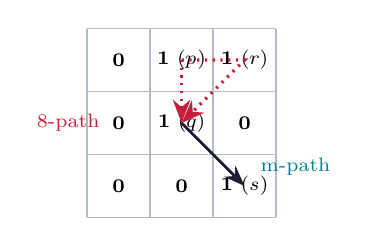
\begin{tikzpicture}[scale=0.8, every node/.style={font=\scriptsize}]
    % 8-path vs m-path grid
    \draw[step=1.0cm, color=mgframe, line width=0.6pt] (0,0) grid (3,3);
    
    \node at (0.5, 2.5) {\textbf{0}};
    \node at (1.5, 2.5) {\textbf{1} ($p$)};
    \node at (2.5, 2.5) {\textbf{1} ($r$)};
    
    \node at (0.5, 1.5) {\textbf{0}};
    \node at (1.5, 1.5) {\textbf{1} ($q$)};
    \node at (2.5, 1.5) {\textbf{0}};
    
    \node at (0.5, 0.5) {\textbf{0}};
    \node at (1.5, 0.5) {\textbf{0}};
    \node at (2.5, 0.5) {\textbf{1} ($s$)};

    % Draw paths
    \draw[redarrow, dotted, line width=1.2pt] (1.5, 2.5) -- (2.5, 2.5) -- (1.5, 1.5);
    \draw[redarrow, dotted, line width=1.2pt] (1.5, 2.5) -- (1.5, 1.5);
    \node[color=myred] at (-0.3, 1.5) {8-path};
    
    % m-path
    \draw[arrow, line width=1pt] (1.5, 1.5) -- (2.5, 0.5);
    \node[color=myteal, right] at (2.6, 0.8) {m-path};
  \end{tikzpicture}
  \par\vspace{2pt}\small\textbf{m-path resolves 8-path ambiguity}
\end{minipage}
\end{tcolorbox}

\subsection{Distance Measures}
Let $p(x,y)$, $q(s,t)$, and $z(v,w)$ be pixels. A distance function $D(p,q)$ must satisfy:
\begin{itemize}[leftmargin=*, itemsep=2pt]
  \item $D(p,q) \ge 0$ ($D(p,q) = 0$ if and only if $p = q$)
  \item $D(p,q) = D(q,p)$ (Symmetry)
  \item $D(p,z) \le D(p,q) + D(q,z)$ (Triangle Inequality)
\end{itemize}

\begin{tcolorbox}[formulabox, title={Key Distance Metrics}]
\textbf{Euclidean Distance ($D_e$):}
\begin{equation}
  D_e(p,q) = \sqrt{(x-s)^2 + (y-t)^2}
\end{equation}
\par\noindent
\textbf{City-Block Distance ($D_4$):}
\begin{equation}
  D_4(p,q) = |x-s| + |y-t|
\end{equation}
\par\noindent
\textbf{Chessboard Distance ($D_8$):}
\begin{equation}
  D_8(p,q) = \max(|x-s|, |y-t|)
\end{equation}
\end{tcolorbox}

% ===============================================================================
\section{Worked Examples}
% ===============================================================================

\begin{tcolorbox}[examplebox, title={Distance Calculations and Path Analysis}]
\textbf{Problem:} Given pixel $p$ at coordinates $(3,4)$ and pixel $q$ at coordinates $(7,8)$ in a digital image:
\begin{enumerate}[label=(\alph*), leftmargin=*, itemsep=2pt]
  \item Calculate the Euclidean distance $D_e(p,q)$.
  \item Calculate the City-Block distance $D_4(p,q)$.
  \item Calculate the Chessboard distance $D_8(p,q)$.
  \item Determine if there is an m-path between $p$ and $q$ using $V = \{1\}$ in the following $3 \times 3$ grid segment, where the coordinates are:
  \begin{center}
    \begin{tabular}{c c c}
      $a(0,2) = 0$ & $b(1,2) = 1$ & $c(2,2) = 1$ \\
      $d(0,1) = 0$ & $e(1,1) = 1$ & $f(2,1) = 0$ \\
      $g(0,0) = 0$ & $h(1,0) = 0$ & $i(2,0) = 1$
    \end{tabular}
  \end{center}
\end{enumerate}

\par\noindent\rule{\linewidth}{0.5pt}\par
\textbf{Solution:}
\par\noindent
\textbf{(a) Euclidean Distance ($D_e$):}
\begin{equation*}
  D_e(p,q) = \sqrt{(3-7)^2 + (4-8)^2} = \sqrt{(-4)^2 + (-4)^2} = \sqrt{16+16} = \sqrt{32} \approx 5.66
\end{equation*}

\textbf{(b) City-Block Distance ($D_4$):}
\begin{equation*}
  D_4(p,q) = |3-7| + |4-8| = 4 + 4 = 8
\end{equation*}

\textbf{(c) Chessboard Distance ($D_8$):}
\begin{equation*}
  D_8(p,q) = \max(|3-7|, |4-8|) = \max(4, 4) = 4
\end{equation*}

\textbf{(d) m-path Analysis:}
\begin{itemize}[leftmargin=*, itemsep=2pt]
  \item We seek a path of pixels with value $1$ between $e(1,1)$ and $i(2,0)$ under m-adjacency rules.
  \item Let's check neighbors of $e(1,1)$:
    \begin{itemize}[leftmargin=1em, itemsep=1.5pt]
      \item $b(1,2)$ has value $1$ and is a 4-neighbor of $e$ ($b \in N_4(e)$). Thus, there is an m-path segment $e \leftrightarrow b$.
      \item $i(2,0)$ is a diagonal neighbor of $e$ ($i \in N_D(e)$).
      \item Under m-adjacency rules, diagonal pixels $e$ and $i$ are m-adjacent only if the intersection of their 4-neighbors has no pixels of value $V=\{1\}$.
      \item $N_4(e) \cap N_4(i) = \{ (2,1), (1,0) \} = \{ f, h \}$.
      \item Since $f(2,1) = 0$ and $h(1,0) = 0$, both intersection pixels have value $0$, which is not in $V$.
      \item Therefore, $e$ and $i$ are directly m-adjacent. The path is $e \leftrightarrow i$ (length 1).
    \end{itemize}
  \item Now let's check path from $b(1,2)$ to $i(2,0)$:
    \begin{itemize}[leftmargin=1em, itemsep=1.5pt]
      \item $c(2,2)$ is in $N_4(b)$ and has value $1$. Thus, $b \leftrightarrow c$.
      \item $i(2,0)$ is a diagonal neighbor of $f$, but $c$ and $i$ are not adjacent. The only valid path is $b \leftrightarrow e \leftrightarrow i$.
    \end{itemize}
\end{itemize}
\end{tcolorbox}

\newpage

% ===============================================================================
% MANDATORY QUICK REVISION PAGE
% ===============================================================================
\begin{center}
  {\large\bfseries\color{myred} Quick Revision --- Module I}\\[3pt]
  {\small\color{mydark} Digital Image Fundamentals $|$ PE-EC702B}
\end{center}
\noindent{\color{myred}\rule{\linewidth}{1.2pt}}
\vspace{4pt}

\begin{tcolorbox}[formulabox, title={\textbf{Key Formulas at a Glance}}]
\renewcommand{\arraystretch}{1.3}
\begin{tabularx}{\linewidth}{B{5.0cm} X}
Quantization Levels & $L = 2^k$ \quad ($k$ = bit depth) \\
Storage Requirement & $b = M \times N \times k$ \quad (bits for an $M \times N$ image) \\
Euclidean Distance & $D_e(p,q) = \sqrt{(x-s)^2 + (y-t)^2}$ \\
City-Block Distance & $D_4(p,q) = |x-s| + |y-t|$ \\
Chessboard Distance & $D_8(p,q) = \max(|x-s|, |y-t|)$ \\
Weber Fraction & $\text{Weber Ratio} = \frac{\Delta I}{I}$ \quad ($\Delta I$ = just noticeable increment)
\end{tabularx}
\end{tcolorbox}

\begin{tcolorbox}[defbox, title={\textbf{One-Line Definitions}}]
\begin{itemize}[leftmargin=*, itemsep=2.5pt, topsep=0pt]
  \item \textbf{Photopic Vision:} Vision mediated by cone cells under bright light, providing high color and spatial resolution.
  \item \textbf{Scotopic Vision:} Vision mediated by rod cells under low light, providing color-blind, coarse spatial vision.
  \item \textbf{Sampling:} Discretizing continuous coordinates $(x,y)$ to define spatial resolution.
  \item \textbf{Quantization:} Discretizing continuous amplitude (gray level) to define intensity resolution.
  \item \textbf{False Contouring:} Artificial banding appearing in regions of smooth transitions due to low quantization.
  \item \textbf{m-Adjacency:} Mixed adjacency that prevents dual-path ambiguities by checking vertical/horizontal neighbors.
\end{itemize}
\end{tcolorbox}

\begin{tcolorbox}[exambox, title={\textbf{Frequently Asked / Viva Questions}}]
\begin{enumerate}[leftmargin=*, itemsep=3.5pt, label=\arabic*.]
  \item \Q{State the difference between rods and cones.} Cones are located mainly in the fovea, are color-sensitive, and operate in bright light (photopic vision). Rods are distributed across the retina, are highly sensitive to low light (scotopic vision), and are color-blind.
  \item \Q{What is Weber ratio? What does a low Weber ratio imply?} It is the ratio of the just noticeable increment in intensity $\Delta I$ to the background intensity $I$. A low Weber ratio implies high intensity discrimination capability of the human eye.
  \item \Q{Why is m-adjacency preferred over 8-adjacency?} 8-adjacency can lead to multiple, ambiguous paths between two pixels (e.g., both diagonal and horizontal-vertical paths simultaneously). m-adjacency resolves this by choosing the diagonal path only when no horizontal-vertical path exists.
  \item \Q{Explain the concept of false contouring.} If the number of quantization levels $L$ is too low (typically $< 16$ levels), the smooth transitions of intensity appear as discrete, nested bands of constant gray level with sharp, artificial boundaries.
  \item \Q{How does city-block distance differ from chessboard distance?} $D_4$ distance (city-block) allows only horizontal and vertical movements, while $D_8$ distance (chessboard) allows both horizontal-vertical and diagonal movements. For any two points, $D_8(p,q) \le D_4(p,q)$.
  \item \Q{What is spatial resolution and how is it measured?} It is the smallest discernible detail in an image. It is measured in terms of line pairs per unit distance or dots per inch (dpi).
  \item \Q{What is the storage size of a $512 \times 512$ image with 256 gray levels?} $256 = 2^8$, so $k = 8$ bits. Total size $b = 512 \times 512 \times 8 = 2,097,152 \text{ bits} = 256 \text{ KB}$.
  \item \Q{What causes aliasing in digital images?} Aliasing occurs when the sampling frequency is less than twice the maximum spatial frequency of the image (violating the Nyquist criterion), causing high-frequency details to wrap as moir\'{e} patterns.
  \item \Q{Define a path between two pixels $p$ and $q$.} A path is a sequence of distinct pixels $(x_0, y_0), (x_1, y_1), \dots, (x_n, y_n)$ where $(x_0, y_0) = p$, $(x_n, y_n) = q$, and $(x_i, y_i)$ is adjacent to $(x_{i-1}, y_{i-1})$ for all $1 \le i \le n$.
  \item \Q{What are the components of an image sensing device?} An image sensing device consists of a filter (to select wavelength band), a sensing material (to convert photon energy to charge), and a readout circuit (to convert charge to voltage).
\end{enumerate}
\tcbset{colbacktitle=myteal, coltitle=white}
\end{tcolorbox}

\begin{tcolorbox}[tikzbox, title={Comparison of Pixel Distances}]
\centering
\renewcommand{\arraystretch}{1.2}
\begin{tabularx}{\linewidth}{>{\bfseries}B{3.5cm} Y Y}
\rowcolor{hdrgray} Distance Metric & Path allowed & Value for $p(0,0)$ and $q(2,2)$ \\
\midrule
Euclidean ($D_e$) & Straight line (any angle) & $\sqrt{2^2 + 2^2} = \sqrt{8} \approx 2.83$ \\
\rowcolor{rowalt} City-Block ($D_4$) & Horizontal and vertical only & $2 + 2 = 4$ \\
Chessboard ($D_8$) & Horizontal, vertical, and diagonal & $\max(2,2) = 2$ \\
\bottomrule
\end{tabularx}
\end{tcolorbox}


% -- Module 2 -----------------------------------------------------------------
\modulestart{2}{Gray Level Transformations}

\section{Gray Level Transformations}
% ===============================================================================

Gray level transformations operate directly on individual pixel values in the spatial domain. The basic mapping function is $s = T(r)$, where $r$ is the input intensity and $s$ is the processed intensity.

\begin{tcolorbox}[defbox, title={Standard Gray Level Mapping Functions}]
\begin{enumerate}[label=\arabic*., leftmargin=*, itemsep=2.5pt]
  \item \textbf{Image Negatives:} Reverses the intensity levels of an image:
    \begin{equation}
      s = L - 1 - r
    \end{equation}
    where $L$ is the number of gray levels. Useful for enhancing white or light detail embedded in dark regions.
  \item \textbf{Log Transformations:} Expands dynamic range of dark pixels while compressing high-level values:
    \begin{equation}
      s = c \log(1 + r)
    \end{equation}
    where $c$ is a constant. Highly useful for displaying Fourier spectra that contain huge intensity ranges.
  \item \textbf{Power-Law (Gamma) Transformations:} Maps a narrow band of dark values into a wider range:
    \begin{equation}
      s = c r^\gamma
    \end{equation}
    where $\gamma$ is the exponent.
    \begin{itemize}[leftmargin=1em, itemsep=1pt]
      \item $\gamma < 1$: Expands dark regions, compresses bright regions.
      \item $\gamma > 1$: Compresses dark regions, expands bright regions.
    \end{itemize}
\end{enumerate}
\end{tcolorbox}

% ===============================================================================
\section{Histogram Processing}
% ===============================================================================

The histogram of a digital image with intensity levels in $[0, L-1]$ is a discrete function $h(r_k) = n_k$, where $n_k$ is the number of pixels with intensity $r_k$.

\subsection{Histogram Equalization}
Histogram equalization is an automated method to improve image contrast by transforming the intensity values such that the output image has a uniform distribution of gray levels.

\begin{tcolorbox}[formulabox, title={Continuous Case Derivation}]
Let $r$ be a continuous variable in $[0, L-1]$. We seek a transformation $s = T(r)$ satisfying:
\begin{enumerate}[label=(\roman*), leftmargin=*, itemsep=1pt]
  \item $T(r)$ is monotonically increasing (preserves intensity order).
  \item $0 \le T(r) \le L-1$ for $0 \le r \le L-1$.
\end{enumerate}
Using probability theory, the probability density function (PDF) of the transformed variable $s$, $p_s(s)$, is:
\begin{equation}
  p_s(s) = p_r(r) \left| \frac{dr}{ds} \right|
\end{equation}
Let us choose the transformation function to be the cumulative distribution function (CDF) of $r$:
\begin{equation}
  s = T(r) = (L-1) \int_0^r p_r(w) \, dw
\end{equation}
Differentiating $s$ with respect to $r$ using the Fundamental Theorem of Calculus:
\begin{equation}
  \frac{ds}{dr} = \frac{dT(r)}{dr} = (L-1) p_r(r)
\end{equation}
Substituting this back into the PDF expression:
\begin{equation}
  p_s(s) = p_r(r) \left| \frac{1}{(L-1) p_r(r)} \right| = \frac{1}{L-1}
\end{equation}
This proves that the resulting PDF $p_s(s)$ is flat (uniform) over the range $[0, L-1]$.
\end{tcolorbox}

For discrete images, the transformation function is:
\begin{equation}
  s_k = T(r_k) = (L-1) \sum_{j=0}^k p_r(r_j) = \frac{L-1}{MN} \sum_{j=0}^k n_j
\end{equation}
where $MN$ is the total number of pixels in the image.

\subsection{Histogram Specification}
Histogram specification allows us to designate the shape of the histogram we wish the processed image to have, rather than just generating a uniform histogram.
\begin{enumerate}[leftmargin=*, itemsep=2.5pt]
  \item Equalize the input image to get $s_k = T(r_k)$.
  \item Compute the transformation function $G(z_q)$ for the specified output histogram:
    \begin{equation}
      v_q = G(z_q) = (L-1)\sum_{i=0}^q p_z(z_i)
    \end{equation}
  \item Perform the inverse mapping: $z_q = G^{-1}(s_k)$.
\end{enumerate}

% ===============================================================================
\section{Spatial Domain Filtering}
% ===============================================================================

Spatial filtering involves moving a filter mask (kernel) over each pixel of an image to perform operations on the pixel neighborhood.

\subsection{Smoothing Filters (Low-pass)}
\begin{itemize}[leftmargin=*, itemsep=3.5pt]
  \item \textbf{Linear Smoothing Filters:} Replacing each pixel by the average of its neighbors (e.g., Box filter, Gaussian filter). Reduces noise but blurs edges.
  \item \textbf{Order-Statistics Filters (Non-linear):} Replacement based on ordering (ranking) the pixels in the neighborhood.
    \begin{itemize}[leftmargin=1.5em, itemsep=1.5pt]
      \item \textbf{Median Filter:} Replaces pixel value with the median of the neighborhood. Excellent for removing \textbf{salt-and-pepper (impulse) noise} while preserving edges.
      \item \textbf{Max/Min Filters:} Replaces with maximum/minimum value (enhances bright/dark details).
    \end{itemize}
\end{itemize}

\subsection{Sharpening Filters (High-pass)}
Sharpening highlights transitions in intensity (edges) using spatial differentiation.
\begin{enumerate}[leftmargin=*, itemsep=3.5pt]
  \item \textbf{First-Derivative Sharpening (Gradient):}
    The gradient magnitude is used to detect edges. The Sobel operator uses two $3 \times 3$ masks to compute horizontal ($G_x$) and vertical ($G_y$) gradients:
    \begin{equation}
      G_x = \begin{bmatrix} -1 & 0 & 1 \\ -2 & 0 & 2 \\ -1 & 0 & 1 \end{bmatrix}, \quad
      G_y = \begin{bmatrix} -1 & -2 & -1 \\ 0 & 0 & 0 \\ 1 & 2 & 1 \end{bmatrix}
    \end{equation}
  \item \textbf{Second-Derivative Sharpening (Laplacian):}
    The isotropic Laplacian operator is defined as:
    \begin{equation}
      \nabla^2 f = \frac{\partial^2 f}{\partial x^2} + \frac{\partial^2 f}{\partial y^2}
    \end{equation}
    The standard discrete Laplacian mask is:
    \begin{equation}
      H = \begin{bmatrix} 0 & 1 & 0 \\ 1 & -4 & 1 \\ 0 & 1 & 0 \end{bmatrix} \quad \text{or} \quad
      H_{\text{diag}} = \begin{bmatrix} 1 & 1 & 1 \\ 1 & -8 & 1 \\ 1 & 1 & 1 \end{bmatrix}
    \end{equation}
\end{enumerate}

% ===============================================================================
\section{Frequency Domain Filtering}
% ===============================================================================

Frequency filtering operates on the 2D Discrete Fourier Transform (DFT) of the image.

\begin{tcolorbox}[tikzbox, title={Spatial vs. Frequency Domain Filtering Flow}]
\centering
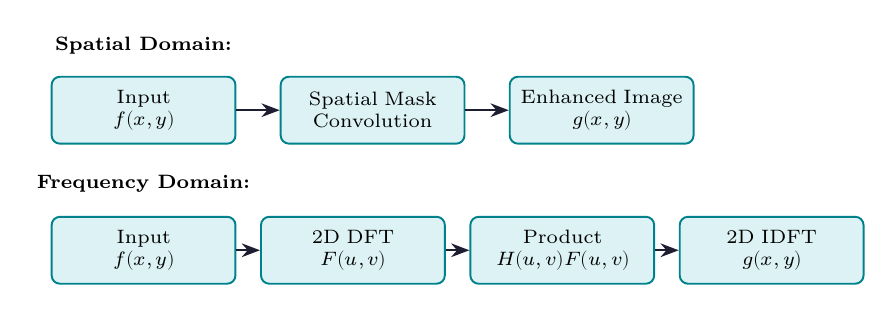
\begin{tikzpicture}[node distance=0.3cm and 0.55cm,
  sblock/.style={rectangle, draw=myteal, fill=hdrteal, text width=2.1cm,
    align=center, minimum height=0.85cm, font=\scriptsize,
    rounded corners=3pt, line width=0.7pt}]

  % Spatial Domain
  \node[font=\scriptsize\bfseries] (lbl1) at (0, 0.75) {Spatial Domain:};
  \node[sblock, below=0.15cm of lbl1] (s_in) {Input\\$f(x,y)$};
  \node[sblock, right=of s_in] (s_filt) {Spatial Mask\\Convolution};
  \node[sblock, right=of s_filt] (s_out) {Enhanced Image\\$g(x,y)$};
  \draw[arrow] (s_in) -- (s_filt);
  \draw[arrow] (s_filt) -- (s_out);

  % Frequency Domain
  \node[font=\scriptsize\bfseries] (lbl2) at (0, -1.0) {Frequency Domain:};
  \begin{scope}[shift={(0, -1.85)}]
    \node[sblock] (f_in) {Input\\$f(x,y)$};
    \node[sblock, right=0.3cm of f_in] (f_dft) {2D DFT\\$F(u,v)$};
    \node[sblock, right=0.3cm of f_dft] (f_mult) {Product\\$H(u,v)F(u,v)$};
    \node[sblock, right=0.3cm of f_mult] (f_idft) {2D IDFT\\$g(x,y)$};
    \draw[arrow] (f_in) -- (f_dft);
    \draw[arrow] (f_dft) -- (f_mult);
    \draw[arrow] (f_mult) -- (f_idft);
  \end{scope}
\end{tikzpicture}
\end{tcolorbox}

Let $D(u,v) = \sqrt{(u - M/2)^2 + (v - N/2)^2}$ be the distance from the center of the frequency rectangle.
\begin{itemize}[leftmargin=*, itemsep=3.5pt]
  \item \textbf{Low-Pass Filters (LPF):} Smooths images by attenuating high frequencies.
    \begin{itemize}[leftmargin=1.5em, itemsep=1.5pt]
      \item \textbf{Ideal LPF:} $H(u,v) = 1$ if $D(u,v) \le D_0$; else $0$. Introduces severe \textbf{ringing artifacts} due to sharp transition.
      \item \textbf{Butterworth LPF (order $n$):} $H(u,v) = \frac{1}{1 + [D(u,v)/D_0]^{2n}}$. Smooth transition, less ringing.
      \item \textbf{Gaussian LPF:} $H(u,v) = e^{-D^2(u,v)/2D_0^2}$. Completely free of ringing.
    \end{itemize}
  \item \textbf{High-Pass Filters (HPF):} Sharpens images (high frequencies are kept, low frequencies attenuated). Formulas are $H_{\text{HPF}}(u,v) = 1 - H_{\text{LPF}}(u,v)$.
\end{itemize}

% ===============================================================================
\section{Worked Examples}
% ===============================================================================

\begin{tcolorbox}[examplebox, title={Discrete Histogram Equalization}]
\textbf{Problem:} Equalize a 3-bit image ($L=8$ levels) of size $64 \times 64$ ($MN = 4096$) with the following gray-level distribution:
\begin{center}
  \small
  \begin{tabular}{c c c c c c c c c}
    \toprule
    Gray Level $r_k$ & 0 & 1 & 2 & 3 & 4 & 5 & 6 & 7 \\
    \midrule
    Pixel count $n_k$ & 790 & 1023 & 850 & 656 & 329 & 245 & 122 & 81 \\
    \bottomrule
  \end{tabular}
\end{center}

\par\noindent\rule{\linewidth}{0.5pt}\par
\textbf{Solution:}
We use the transformation formula: $s_k = \text{round}\left( (L-1) \sum_{j=0}^k \frac{n_j}{MN} \right) = \text{round}\left( \frac{7}{4096} \sum_{j=0}^k n_j \right)$.
Let's compute the cumulative sum and map the values step-by-step:

\begin{enumerate}[leftmargin=*, itemsep=3.5pt]
  \item \textbf{For $k=0$ ($r_0 = 0$):}
    Cumulative sum $\sum = 790$.
    $s_0 = \frac{7}{4096} \times 790 = 1.35 \rightarrow \text{round}(1.35) = 1$.
  \item \textbf{For $k=1$ ($r_1 = 1$):}
    Cumulative sum $\sum = 790 + 1023 = 1813$.
    $s_1 = \frac{7}{4096} \times 1813 = 3.10 \rightarrow \text{round}(3.10) = 3$.
  \item \textbf{For $k=2$ ($r_2 = 2$):}
    Cumulative sum $\sum = 1813 + 850 = 2663$.
    $s_2 = \frac{7}{4096} \times 2663 = 4.55 \rightarrow \text{round}(4.55) = 5$.
  \item \textbf{For $k=3$ ($r_3 = 3$):}
    Cumulative sum $\sum = 2663 + 656 = 3319$.
    $s_3 = \frac{7}{4096} \times 3319 = 5.67 \rightarrow \text{round}(5.67) = 6$.
  \item \textbf{For $k=4$ ($r_4 = 4$):}
    Cumulative sum $\sum = 3319 + 329 = 3648$.
    $s_4 = \frac{7}{4096} \times 3648 = 6.23 \rightarrow \text{round}(6.23) = 6$.
  \item \textbf{For $k=5$ ($r_5 = 5$):}
    Cumulative sum $\sum = 3648 + 245 = 3893$.
    $s_5 = \frac{7}{4096} \times 3893 = 6.65 \rightarrow \text{round}(6.65) = 7$.
  \item \textbf{For $k=6$ ($r_6 = 6$):}
    Cumulative sum $\sum = 3893 + 122 = 4015$.
    $s_6 = \frac{7}{4096} \times 4015 = 6.86 \rightarrow \text{round}(6.86) = 7$.
  \item \textbf{For $k=7$ ($r_7 = 7$):}
    Cumulative sum $\sum = 4015 + 81 = 4096$.
    $s_7 = \frac{7}{4096} \times 4096 = 7.00 \rightarrow \text{round}(7.00) = 7$.
\end{enumerate}

\par\noindent\textbf{Final Intensity Mapping Summary:}
\begin{center}
  \small
  \begin{tabular}{c c c c c c c c c}
    \toprule
    Original $r_k$ & 0 & 1 & 2 & 3 & 4 & 5 & 6 & 7 \\
    Mapped $s_k$   & 1 & 3 & 5 & 6 & 6 & 7 & 7 & 7 \\
    New Count      & 790 & 1023 & 850 & 985 & 0 & 448 & 0 & 0 \\
    \bottomrule
  \end{tabular}
\end{center}
Note that the output gray levels are now spread out over $[1,7]$, which significantly enhances contrast.
\end{tcolorbox}

\newpage

% ===============================================================================
% MANDATORY QUICK REVISION PAGE
% ===============================================================================
\begin{center}
  {\large\bfseries\color{myred} Quick Revision --- Module II}\\[3pt]
  {\small\color{mydark} Image Enhancements and Filtering $|$ PE-EC702B}
\end{center}
\noindent{\color{myred}\rule{\linewidth}{1.2pt}}
\vspace{4pt}

\begin{tcolorbox}[formulabox, title={\textbf{Key Formulas at a Glance}}]
\renewcommand{\arraystretch}{1.3}
\begin{tabularx}{\linewidth}{B{5.0cm} X}
Image Negative & $s = L - 1 - r$ \\
Power-Law (Gamma) & $s = c r^\gamma$ \\
Histogram Equalization & $s_k = \frac{L-1}{MN} \sum_{j=0}^k n_j$ \\
Laplacian Mask Operator & $\nabla^2 f(x,y) = f(x+1,y)+f(x-1,y)+f(x,y+1)+f(x,y-1)-4f(x,y)$ \\
2D DFT & $F(u,v) = \sum_{x=0}^{M-1} \sum_{y=0}^{N-1} f(x,y) e^{-j2\pi(\frac{ux}{M} + \frac{vy}{N})}$ \\
Gaussian Low-Pass Filter & $H(u,v) = e^{-D^2(u,v)/2D_0^2}$
\end{tabularx}
\end{tcolorbox}

\begin{tcolorbox}[defbox, title={\textbf{One-Line Definitions}}]
\begin{itemize}[leftmargin=*, itemsep=2.5pt, topsep=0pt]
  \item \textbf{Median Filtering:} A non-linear spatial enhancement technique that is robust against impulse noise while preserving edges.
  \item \textbf{Isotropic Operator:} A differential operator whose response is independent of the direction of the transitions.
  \item \textbf{Ringing Artifact:} Ripple patterns appearing near sharp boundaries in images filtered with Ideal LPFs due to Gibbs phenomenon.
  \item \textbf{Histogram Equalization:} A method that enhances contrast by transforming the intensity values to achieve a uniform PDF.
  \item \textbf{Sobel Operator:} A first-derivative edge detection operator utilizing gradient masks to compute directional differences.
  \item \textbf{Frequency Domain Filtering:} Modifying the Fourier coefficients of an image before performing the inverse transform.
\end{itemize}
\end{tcolorbox}

\begin{tcolorbox}[exambox, title={\textbf{Frequently Asked / Viva Questions}}]
\begin{enumerate}[leftmargin=*, itemsep=3.5pt, label=\arabic*.]
  \item \Q{What is the effect of choosing $\gamma < 1$ in power-law transformation?} It expands the dark regions of the image (revealing details in shadows) and compresses the brighter regions.
  \item \Q{Why does the Ideal LPF produce ringing artifacts while the Gaussian LPF does not?} The transfer function of an Ideal LPF has a sharp discontinuity in the frequency domain, whose Fourier inverse is a sinc function containing spatial oscillations. The Gaussian LPF has smooth Gaussian transitions in both domains, eliminating oscillations.
  \item \Q{Which filter is best suited for salt-and-pepper noise? Why?} The Median filter, because the impulse noise pixels represent outlier values which are completely discarded when the neighborhood values are ranked.
  \item \Q{Write down the basic difference between correlation and convolution.} In spatial correlation, the filter mask is directly multiplied and summed with the image. In convolution, the mask is rotated by $180^\circ$ before multiplying and summing.
  \item \Q{How does the Laplacian filter sharpen an image?} The Laplacian computes the second derivative, highlighting rapid intensity transitions (edges). By subtracting the Laplacian from the original image ($g(x,y) = f(x,y) - \nabla^2 f(x,y)$), the edges are enhanced.
  \item \Q{State the difference between histogram equalization and histogram specification.} Histogram equalization automatically spreads the intensity levels uniformly, while histogram specification maps the image to a user-defined target histogram shape.
  \item \Q{What are Butterworth filters?} Butterworth filters have a transfer function with a transition band whose sharpness is controlled by the order parameter $n$, striking a balance between Ideal LPF (sharp transition) and Gaussian LPF (very smooth transition).
  \item \Q{Why do we shift the origin of the 2D DFT before filtering?} Shifting the origin (using $f(x,y)(-1)^{x+y}$) centers the low-frequency component $F(0,0)$ at the center of the frequency rectangle, simplifying filter design.
  \item \Q{Define the gradient of an image $f(x,y)$.} The gradient is a 2D vector $\nabla f = \left[ \frac{\partial f}{\partial x}, \frac{\partial f}{\partial y} \right]^T$ that points in the direction of the maximum rate of change of intensity.
  \item \Q{What is frequency domain high-pass filtering?} HPF attenuates the low frequencies (representing smooth variations) while passing the high frequencies (representing edges and noise), resulting in sharpened details.
\end{enumerate}
\tcbset{colbacktitle=myteal, coltitle=white}
\end{tcolorbox}

\begin{tcolorbox}[tikzbox, title={Comparison of Sharpening Operators}]
\centering
\renewcommand{\arraystretch}{1.2}
\begin{tabularx}{\linewidth}{>{\bfseries}B{3.5cm} Y Y}
\rowcolor{hdrgray} Attribute & First-Derivative (Gradient) & Second-Derivative (Laplacian) \\
\midrule
Response at Constant & Zero response & Zero response \\
\rowcolor{rowalt} Response at Step/Ramp & Non-zero along the ramp & Non-zero only at start/end of ramp \\
Ramp Response Width & Produces thick, double-pixel edges & Produces thin, single-pixel edges \\
\bottomrule
\end{tabularx}
\tcbset{colbacktitle=myteal, coltitle=white}
\end{tcolorbox}


% -- Module 3 -----------------------------------------------------------------
\modulestart{3}{Color Models}

\section{Color Models}
% ===============================================================================

Color models provide a standardized way to specify colors. They are typically categorized as hardware-oriented (RGB, YUV) or human-oriented (HSI).

\subsection{RGB Color Model}
The RGB model is based on a 3D Cartesian coordinate system where the primary colors Red, Green, and Blue are at three corners. The values are typically normalized to $[0,1]$:
\begin{itemize}[leftmargin=*, itemsep=2pt]
  \item Black is at the origin $(0,0,0)$, while White is at $(1,1,1)$.
  \item Colors are additive: combining primaries yields secondary colors (Cyan, Magenta, Yellow).
\end{itemize}

\subsection{YUV Color Model}
Used widely in television transmission and video compression standards (like MPEG/H.26X). It decouples brightness (Luminance) from color (Chrominance):
\begin{itemize}[leftmargin=*, itemsep=3.5pt]
  \item \textbf{Y (Luminance):} Represents brightness information.
  \item \textbf{U and V (Chrominance):} Represent color differences.
  \item Conversion from RGB to YUV:
    \begin{align}
      Y &= 0.299R + 0.587G + 0.114B \\
      U &= -0.14713R - 0.28886G + 0.436B \approx 0.492(B - Y) \\
      V &= 0.615R - 0.51499G - 0.10001B \approx 0.877(R - Y)
    \end{align}
\end{itemize}

\subsection{HSI Color Model}
The HSI model decouples intensity from color-carrying information, matching human visual perception.

\begin{tcolorbox}[defbox, title={HSI Components}]
\begin{itemize}[leftmargin=*, itemsep=3pt]
  \item \textbf{Hue (H):} Describes the pure color (e.g., yellow, red, purple) represented as an angle from $0^\circ$ to $360^\circ$.
  \item \textbf{Saturation (S):} Represents the purity or dilution of the color with white (range $[0,1]$).
  \item \textbf{Intensity (I):} Represents the brightness or gray-level value (range $[0,1]$).
\end{itemize}
\end{tcolorbox}

\begin{tcolorbox}[formulabox, title={RGB to HSI Conversion Formulas}]
Given $R, G, B \in [0, 1]$, the HSI components are computed as:
\begin{align}
  I &= \frac{1}{3}(R + G + B) \\
  S &= 1 - \frac{3}{R + G + B} \left[ \min(R, G, B) \right] \\
  H &= \begin{cases} \theta & \text{if } B \le G \\ 360^\circ - \theta & \text{if } B > G \end{cases}
\end{align}
where the angle $\theta$ is:
\begin{equation}
  \theta = \cos^{-1} \left( \frac{\frac{1}{2}\left[(R - G) + (R - B)\right]}{\sqrt{(R - G)^2 + (R - B)(G - B)}} \right)
\end{equation}
\end{tcolorbox}

\begin{tcolorbox}[tikzbox, title={HSI Color Model Coordinates}]
\centering
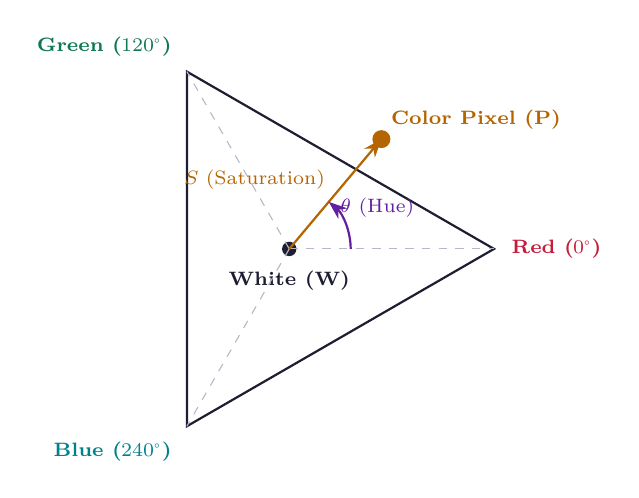
\begin{tikzpicture}[scale=1.3, every node/.style={font=\scriptsize}]
  % Draw RGB triangle on the chromaticity plane
  \draw[thick, color=mydark] (0:2) coordinate (R) -- (120:2) coordinate (G) -- (240:2) coordinate (B) -- cycle;
  
  % Label vertices
  \node[right=0.1cm, color=myred] at (R) {\textbf{Red ($0^\circ$)}};
  \node[above left=0.1cm, color=mygreen] at (G) {\textbf{Green ($120^\circ$)}};
  \node[below left=0.1cm, color=myteal] at (B) {\textbf{Blue ($240^\circ$)}};
  
  % Center point (White)
  \fill[color=mydark] (0,0) circle (2pt) node[below=0.15cm] {\textbf{White (W)}};
  
  % Draw lines from center to vertices
  \draw[dashed, color=mgframe] (0,0) -- (R);
  \draw[dashed, color=mgframe] (0,0) -- (G);
  \draw[dashed, color=mgframe] (0,0) -- (B);
  
  % Draw an arbitrary color point P
  \coordinate (P) at (50:1.4);
  \fill[color=myamber] (P) circle (2.5pt) node[above right] {\textbf{Color Pixel (P)}};
  \draw[thick, -Stealth, color=myamber] (0,0) -- (P) node[midway, above left, yshift=-2pt] {$S$ (Saturation)};
  
  % Draw Hue angle arc from 0 to 50 degrees
  \draw[thick, color=mypurple, -Stealth] (0:0.6) arc (0:50:0.6);
  \node[color=mypurple] at (25:0.95) {$\theta$ (Hue)};
\end{tikzpicture}
\end{tcolorbox}

% ===============================================================================
\section{Color Transformations}
% ===============================================================================

Color transformations map input color pixels $\mathbf{r}$ to output pixels $\mathbf{s}$:
\begin{equation}
  s_i = T_i(r_1, r_2, \dots, r_n) \quad \text{for } i = 1, 2, \dots, n
\end{equation}
where $n$ is the number of color space dimensions (e.g., $n=3$ for RGB/HSI).

\subsection{Formulations and Corrections}
\begin{itemize}[leftmargin=*, itemsep=3.5pt]
  \item \textbf{Color Complements:} Analogous to gray-scale negatives. In RGB space, the complement is obtained by subtracting the color values from the maximum:
    \begin{equation}
      s_R = 1 - r_R, \quad s_G = 1 - r_G, \quad s_B = 1 - r_B
    \end{equation}
    Useful for enhancing dark details in color images.
  \item \textbf{Color Slicing:} Highlights a specific range of colors in an image while background is set to gray. A prototype color vector $\mathbf{a}$ and distance threshold $D_0$ are defined:
    \begin{equation}
      s_i = \begin{cases} r_i & \text{if } \|\mathbf{z} - \mathbf{a}\| \le D_0 \\ 0.5 & \text{if } \|\mathbf{z} - \mathbf{a}\| > D_0 \end{cases}
    \end{equation}
  \item \textbf{Tone and Color Corrections:} Adjusting brightness, contrast, and gamma on color channels. Applying gamma correction on Intensity ($I$) in HSI space preserves the original hue and saturation, avoiding unwanted color shifts that occur when applying it directly on individual RGB channels.
\end{itemize}

% ===============================================================================
\section{Color Image Smoothing and Sharpening}
% ===============================================================================

\subsection{Color Image Smoothing}
Smoothing can be performed either in full-color vector space or by processing individual channels separately.
\par\noindent
For a neighborhood $S_{xy}$, the average vector is:
\begin{equation}
  \bar{\mathbf{c}}(x,y) = \frac{1}{K}\sum_{(s,t)\in S_{xy}} \mathbf{c}(s,t) = \begin{bmatrix}
    \frac{1}{K}\sum r_R(s,t) \\
    \frac{1}{K}\sum r_G(s,t) \\
    \frac{1}{K}\sum r_B(s,t)
  \end{bmatrix}
\end{equation}
Since vector addition is performed component-wise, smoothing each RGB channel independently yields the exact same result as full-color vector smoothing.

\subsection{Color Image Sharpening}
Sharpening utilizes the Laplacian operator. In RGB vector space:
\begin{equation}
  \nabla^2 \mathbf{c}(x,y) = \begin{bmatrix}
    \nabla^2 c_R(x,y) \\
    \nabla^2 c_G(x,y) \\
    \nabla^2 c_B(x,y)
  \end{bmatrix}
\end{equation}
Like smoothing, color sharpening can be executed by applying the Laplacian operator independently to the Red, Green, and Blue channels.

% ===============================================================================
\section{Color Segmentation}
% ===============================================================================

Color segmentation partitions an image into regions based on color features.

\subsection{Segmentation in RGB Space}
Given a sample set of prototype pixels representing the target color, we compute their mean vector $\mathbf{a}$ and covariance matrix $\mathbf{C}$.
\begin{itemize}[leftmargin=*, itemsep=3.5pt]
  \item \textbf{Euclidean Distance Classifier:} If color features are uncorrelated, we classify pixel $\mathbf{z}$ based on Euclidean distance:
    \begin{equation}
      D(\mathbf{z}, \mathbf{a}) = \|\mathbf{z} - \mathbf{a}\| = \sqrt{(z_R - a_R)^2 + (z_G - a_G)^2 + (z_B - a_B)^2}
    \end{equation}
    A pixel is segmented if $D(\mathbf{z}, \mathbf{a}) \le D_0$.
  \item \textbf{Mahalanobis Distance Classifier:} Accounts for correlations between channels:
    \begin{equation}
      D_M(\mathbf{z}, \mathbf{a}) = \sqrt{(\mathbf{z} - \mathbf{a})^T \mathbf{C}^{-1} (\mathbf{z} - \mathbf{a})}
    \end{equation}
\end{itemize}

\subsection{Segmentation in HSI Space}
Typically performed by thresholding Hue ($H$) and Saturation ($S$) channels:
\begin{itemize}[leftmargin=*, itemsep=2pt]
  \item Intensity is often ignored, making the segmentation robust to illumination variations and shadows.
\end{itemize}

% ===============================================================================
\section{Worked Examples}
% ===============================================================================

\begin{tcolorbox}[examplebox, title={RGB to HSI Conversion}]
\textbf{Problem:} Convert the normalized RGB pixel color vector $\mathbf{c} = [0.2, 0.8, 0.4]^T$ to HSI coordinates.

\par\noindent\rule{\linewidth}{0.5pt}\par
\textbf{Solution:}
Given $R = 0.2$, $G = 0.8$, $B = 0.4$.

\textbf{1. Calculate Intensity (I):}
\begin{equation*}
  I = \frac{1}{3}(R + G + B) = \frac{1}{3}(0.2 + 0.8 + 0.4) = \frac{1.4}{3} \approx 0.467
\end{equation*}

\textbf{2. Calculate Saturation (S):}
First, find $\min(R,G,B) = \min(0.2, 0.8, 0.4) = 0.2$.
\begin{equation*}
  S = 1 - \frac{3}{R + G + B} \left[ \min(R, G, B) \right] = 1 - \frac{3}{1.4}(0.2) = 1 - \frac{0.6}{1.4} = 1 - 0.429 = 0.571
\end{equation*}

\textbf{3. Calculate Hue (H):}
First, calculate the angle $\theta$:
\begin{align*}
  \text{Numerator} &= \frac{1}{2} \left[ (R - G) + (R - B) \right] = \frac{1}{2} \left[ (0.2 - 0.8) + (0.2 - 0.4) \right] \\
  &= \frac{1}{2} \left[ -0.6 - 0.2 \right] = -0.4 \\[4pt]
  \text{Denominator} &= \sqrt{(R-G)^2 + (R-B)(G-B)} = \sqrt{(0.2-0.8)^2 + (0.2-0.4)(0.8-0.4)} \\
  &= \sqrt{(-0.6)^2 + (-0.2)(0.4)} = \sqrt{0.36 - 0.08} = \sqrt{0.28} \approx 0.529
\end{align*}
Compute $\cos\theta$:
\begin{equation*}
  \cos\theta = \frac{-0.4}{0.529} \approx -0.756
\end{equation*}
Therefore:
\begin{equation*}
  \theta = \cos^{-1}(-0.756) \approx 139.1^\circ
\end{equation*}
Since $B = 0.4$ and $G = 0.8$, we have $B \le G$. Thus, Hue is:
\begin{equation*}
  H = \theta = 139.1^\circ
\end{equation*}

\par\noindent\textbf{Final Result:}
The HSI coordinate is:
\begin{equation*}
  H = 139.1^\circ, \quad S = 0.571, \quad I = 0.467
\end{equation*}
\end{tcolorbox}

\newpage

% ===============================================================================
% MANDATORY QUICK REVISION PAGE
% ===============================================================================
\begin{center}
  {\large\bfseries\color{myred} Quick Revision --- Module III}\\[3pt]
  {\small\color{mydark} Color Image Processing $|$ PE-EC702B}
\end{center}
\noindent{\color{myred}\rule{\linewidth}{1.2pt}}
\vspace{4pt}

\begin{tcolorbox}[formulabox, title={\textbf{Key Formulas at a Glance}}]
\renewcommand{\arraystretch}{1.3}
\begin{tabularx}{\linewidth}{B{5.0cm} X}
Intensity (HSI) & $I = \frac{1}{3}(R + G + B)$ \\
Saturation (HSI) & $S = 1 - \frac{3}{R + G + B} \left[ \min(R, G, B) \right]$ \\
Luminance (YUV) & $Y = 0.299R + 0.587G + 0.114B$ \\
RGB Color Complement & $s_R = 1 - r_R, \quad s_G = 1 - r_G, \quad s_B = 1 - r_B$ \\
RGB Euclidean distance & $D(\mathbf{z}, \mathbf{a}) = \sqrt{(z_R - a_R)^2 + (z_G - a_G)^2 + (z_B - a_B)^2}$ \\
Mahalanobis distance & $D_M(\mathbf{z}, \mathbf{a}) = \sqrt{(\mathbf{z} - \mathbf{a})^T \mathbf{C}^{-1} (\mathbf{z} - \mathbf{a})}$
\end{tabularx}
\tcbset{colbacktitle=myteal, coltitle=white}
\end{tcolorbox}

\begin{tcolorbox}[defbox, title={\textbf{One-Line Definitions}}]
\begin{itemize}[leftmargin=*, itemsep=2.5pt, topsep=0pt]
  \item \textbf{Additive Color Model:} Model (like RGB) where primary light sources are added together to create other colors.
  \item \textbf{Hue:} An attribute associated with the dominant wavelength in a mixture of light waves, representing pure color.
  \item \textbf{Saturation:} A measure of the relative purity of a color, indicating how much white light is mixed with it.
  \item \textbf{Color Slicing:} A transformation that isolates a sample color band in an image by zeroing out distant color vectors.
  \item \textbf{Full-Color Processing:} Processing pixels directly as multi-dimensional color vectors rather than scalar components.
  \item \textbf{Chrominance:} The color-carrying portion of a video signal, represented by U and V components in YUV.
\end{itemize}
\end{tcolorbox}

\begin{tcolorbox}[exambox, title={\textbf{Frequently Asked / Viva Questions}}]
\begin{enumerate}[leftmargin=*, itemsep=3.5pt, label=\arabic*.]
  \item \Q{Why is the HSI color model preferred over RGB for human interface design?} Because HSI decouples intensity (brightness) from color features (hue/saturation), which mimics how the human brain perceives and describes colors.
  \item \Q{Which color model is used in video/television broadcasting? Why?} YUV (or $\text{YC}_b\text{C}_r$), because it separates luminance ($Y$) from chrominance. This allows compatible broadcasting to black-and-white TVs and compression of color bandwidth without affecting perceived quality.
  \item \Q{Can we smooth a color image by filtering RGB channels independently?} Yes. Since the average of vectors is equal to the vector containing the averages of their components, independent channel filtering produces mathematically identical results to full-color vector smoothing.
  \item \Q{What is the complement of Red in RGB space?} Under normalized RGB space, Red is $(1,0,0)$. Its complement is $(1-1, 1-0, 1-0) = (0,1,1)$, which represents Cyan (a secondary color).
  \item \Q{What is the main advantage of segmenting color images in HSI space?} By thresholding only Hue ($H$) and Saturation ($S$) and ignoring Intensity ($I$), the segmentation becomes robust to shadows and spatial variations in lighting.
  \item \Q{Explain the physical meaning of a Saturation value of 0.} A saturation of 0 means the color is completely diluted with white light, representing a neutral shade of gray.
  \item \Q{Why do we apply gamma correction to the Intensity channel in HSI rather than RGB channels?} Applying it to RGB channels independently alters their relative ratios, causing severe shifts in hue. Correcting the Intensity channel in HSI preserves hue and saturation.
  \item \Q{What is the difference between Euclidean and Mahalanobis distance in RGB segmentation?} Euclidean distance assumes all color channels are independent and have equal variance. Mahalanobis distance uses the covariance matrix to account for channel correlations.
  \item \Q{What are subtractive primary colors?} Cyan, Magenta, and Yellow. They are used in color printing and act as filters that absorb specific wavelengths of light.
  \item \Q{What does the angle $\theta$ represent in HSI?} The angle $\theta$ represents the starting hue reference vector. It is measured counterclockwise starting from the Red axis ($0^\circ$).
\end{enumerate}
\tcbset{colbacktitle=myteal, coltitle=white}
\end{tcolorbox}

\begin{tcolorbox}[tikzbox, title={Comparison of Color Models}]
\centering
\renewcommand{\arraystretch}{1.2}
\begin{tabularx}{\linewidth}{>{\bfseries}B{3.2cm} Y Y Y}
\rowcolor{hdrgray} Attribute & RGB & YUV & HSI \\
\midrule
Primary Focus & Hardware (displays) & Video coding/TV & Human perception \\
\rowcolor{rowalt} Components & Red, Green, Blue & Luminance, Chrominance & Hue, Saturation, Intensity \\
Decoupled Brightness & No & Yes (via $Y$) & Yes (via $I$) \\
\bottomrule
\end{tabularx}
\tcbset{colbacktitle=myteal, coltitle=white}
\end{tcolorbox}


% -- Module 4 -----------------------------------------------------------------
\modulestart{4}{Detection of Discontinuities}

\section{Detection of Discontinuities}
% ===============================================================================

Image segmentation is based on one of two basic properties of intensity values: discontinuity (partitioning based on abrupt changes) or similarity (partitioning into homogeneous regions).

\begin{tcolorbox}[defbox, title={Edge and Line Detection}]
\textbf{Edge Detection:} The process of locating boundaries where intensity changes rapidly. These are classified as step edges (ideal abrupt transitions) or ramp edges (gradual, practical transitions due to blur).
\end{tcolorbox}

\subsection{Canny Edge Detection Algorithm}
The Canny detector is considered the optimal edge detector due to its low error rate, precise edge localization, and single response constraint.
\begin{enumerate}[leftmargin=*, itemsep=3.5pt]
  \item \textbf{Noise Reduction:} Smooth the image with a 2D Gaussian filter to eliminate high-frequency noise.
  \item \textbf{Gradient Computation:} Compute the local gradient magnitude $M(x,y)$ and direction $\alpha(x,y)$ using Sobel or Prewitt masks.
  \item \textbf{Non-Maximum Suppression (NMS):} Thin the thick edges by checking if the gradient magnitude at a pixel is a local maximum in the direction of the gradient. If not, set it to zero.
  \item \textbf{Hysteresis Thresholding:} Use two thresholds, $T_{\text{high}}$ and $T_{\text{low}}$:
    \begin{itemize}[leftmargin=1em, itemsep=1pt]
      \item Pixels $> T_{\text{high}}$ are marked as strong edges (always kept).
      \item Pixels $< T_{\text{low}}$ are suppressed.
      \item Pixels in-between are marked as weak edges and kept only if they are connected to a strong edge.
    \end{itemize}
\end{enumerate}

% ===============================================================================
\section{Edge Linking and Boundary Detection}
% ===============================================================================

Since noise and lighting can cause breaks in detected edges, edge linking is used to group pixels into meaningful boundaries.

\subsection{Hough Transform}
The Hough Transform groups edge pixels by determining if they lie on a curve of specified shape (typically a straight line).

\begin{tcolorbox}[formulabox, title={Hough Transform Formulations}]
A straight line in Cartesian coordinates is $y = mx + c$.
\par\noindent
In Hough parameter space, every point $(x,y)$ maps to a line in $(m,c)$ space:
\begin{equation}
  c = -x m + y
\end{equation}
However, vertical lines have infinite slope ($m \to \infty$). To resolve this, we use the polar representation:
\begin{equation}
  \rho = x \cos\theta + y \sin\theta
\end{equation}
where $\rho$ is the perpendicular distance from the origin to the line, and $\theta$ is the angle of the normal vector relative to the $x$-axis.
\par\noindent
\textbf{Algorithm:}
\begin{enumerate}[leftmargin=*, itemsep=2pt]
  \item Quantize the parameter space $(\rho, \theta)$ into an accumulator grid.
  \item For each edge pixel $(x_i, y_i)$ in the image, vary $\theta$ over the range $[-90^\circ, 90^\circ]$ and compute the corresponding $\rho$.
  \item Increment the accumulator cell: $A(\rho, \theta) = A(\rho, \theta) + 1$.
  \item Local maxima (peaks) in the accumulator grid indicate lines in the image.
\end{enumerate}
\end{tcolorbox}

% ===============================================================================
\section{Thresholding}
% ===============================================================================

Thresholding converts a grayscale image $f(x,y)$ into a binary image $g(x,y)$ based on intensity.

\subsection{Global vs. Local Adaptive Thresholding}
\begin{itemize}[leftmargin=*, itemsep=3.5pt]
  \item \textbf{Global Thresholding:} A single threshold $T$ is used for the entire image:
    \begin{equation}
      g(x,y) = \begin{cases} 1 & \text{if } f(x,y) > T \\ 0 & \text{if } f(x,y) \le T \end{cases}
    \end{equation}
    Only effective if the image has a bimodal histogram and uniform illumination.
  \item \textbf{Local/Adaptive Thresholding:} The threshold $T(x,y)$ changes dynamically across the image based on local neighborhood statistics (e.g., local mean or local standard deviation), resolving non-uniform illumination.
\end{itemize}

\subsection{Otsu's Optimum Thresholding Method}
Otsu's method automatically selects the optimal global threshold $T$ by maximizing the \textbf{between-class variance} $\sigma_B^2$ of the two pixel classes (background $C_1$ and foreground $C_2$).

\begin{tcolorbox}[formulabox, title={Otsu's Formulation}]
Let $P_1(T)$ and $P_2(T)$ be the probabilities of the two classes separated by threshold $T$, and let $\mu_1(T)$ and $\mu_2(T)$ be their mean intensities.
\par\noindent
The between-class variance $\sigma_B^2(T)$ is defined as:
\begin{equation}
  \sigma_B^2(T) = P_1(T) P_2(T) \left[ \mu_1(T) - \mu_2(T) \right]^2
\end{equation}
We evaluate $\sigma_B^2(T)$ for all possible gray levels $T \in [0, L-1]$. The optimum threshold $T^*$ is the value that maximizes this variance:
\begin{equation}
  T^* = \arg\max_{0 \le T \le L-1} \sigma_B^2(T)
\end{equation}
\end{tcolorbox}

% ===============================================================================
\section{Region-Based Segmentation}
% ===============================================================================

Region-based segmentation groups pixels directly into regions based on similarity.

\begin{itemize}[leftmargin=*, itemsep=3.5pt]
  \item \textbf{Region Growing:} Starts with seed points and appends adjacent pixels to the region if they satisfy homogeneity criteria (e.g., color, texture, intensity).
  \item \textbf{Region Splitting and Merging:}
    \begin{itemize}[leftmargin=1em, itemsep=1.5pt]
      \item Start with the entire image region $R$.
      \item If $R$ does not satisfy the homogeneity criterion $P(R) = \text{True}$ (e.g., variance too high), split it into four disjoint quadrants.
      \item Recursively split non-homogeneous quadrants. This is modeled by a \textbf{quadtree} hierarchy.
      \item After splitting ceases, merge adjacent quadrants $R_i$ and $R_j$ if their union satisfies the homogeneity criterion ($P(R_i \cup R_j) = \text{True}$).
    \end{itemize}
\end{itemize}

\begin{tcolorbox}[tikzbox, title={Quadtree Decomposition for Splitting and Merging}]
\centering
\begin{minipage}{0.42\textwidth}
  \centering
  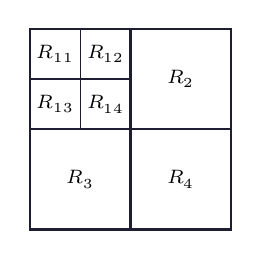
\begin{tikzpicture}[scale=0.85, every node/.style={font=\scriptsize}]
    % Partitioned Image
    \draw[thick, color=mydark] (0,0) rectangle (3,3);
    \draw[thick, color=mydark] (1.5,0) -- (1.5,3);
    \draw[thick, color=mydark] (0,1.5) -- (3,1.5);
    
    % Split top-left block (R1) into 4
    \draw[thin, color=mydark] (0.75, 1.5) -- (0.75, 3.0);
    \draw[thin, color=mydark] (0, 2.25) -- (1.5, 2.25);
    
    % Labels
    \node at (0.375, 2.625) {$R_{11}$};
    \node at (1.125, 2.625) {$R_{12}$};
    \node at (0.375, 1.875) {$R_{13}$};
    \node at (1.125, 1.875) {$R_{14}$};
    \node at (2.25, 2.25) {$R_2$};
    \node at (0.75, 0.75) {$R_3$};
    \node at (2.25, 0.75) {$R_4$};
  \end{tikzpicture}
  \par\vspace{2pt}\small\textbf{Image Partitions}
\end{minipage}
\hfill
\begin{minipage}{0.54\textwidth}
  \centering
  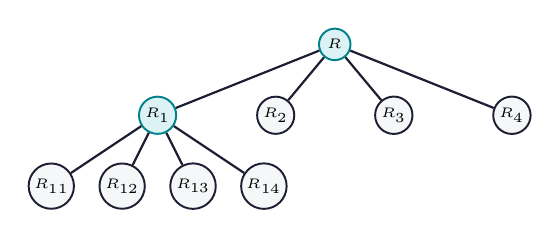
\begin{tikzpicture}[scale=1.0, every node/.style={font=\scriptsize}]
    \tikzset{
      tnode/.style={circle, draw=myteal, fill=hdrteal, minimum size=0.4cm, inner sep=1.2pt, font=\tiny\bfseries, line width=0.7pt},
      leaf/.style={circle, draw=mydark, fill=mygray, minimum size=0.4cm, inner sep=1.2pt, font=\tiny, line width=0.7pt}
    }
    
    % Root Node
    \node[tnode] (root) at (0,0) {$R$};
    
    % Level 1
    \node[tnode] (r1) at (-2.25, -0.9) {$R_1$};
    \node[leaf]  (r2) at (-0.75, -0.9) {$R_2$};
    \node[leaf]  (r3) at (0.75, -0.9) {$R_3$};
    \node[leaf]  (r4) at (2.25, -0.9) {$R_4$};
    
    \draw[line] (root) -- (r1);
    \draw[line] (root) -- (r2);
    \draw[line] (root) -- (r3);
    \draw[line] (root) -- (r4);
    
    % Level 2 (under R1)
    \node[leaf] (r11) at (-3.6, -1.8) {$R_{11}$};
    \node[leaf] (r12) at (-2.7, -1.8) {$R_{12}$};
    \node[leaf] (r13) at (-1.8, -1.8) {$R_{13}$};
    \node[leaf] (r14) at (-0.9, -1.8) {$R_{14}$};
    
    \draw[line] (r1) -- (r11);
    \draw[line] (r1) -- (r12);
    \draw[line] (r1) -- (r13);
    \draw[line] (r1) -- (r14);
  \end{tikzpicture}
  \par\vspace{2pt}\small\textbf{Quadtree Hierarchy}
\end{minipage}
\end{tcolorbox}

% ===============================================================================
\section{Worked Examples}
% ===============================================================================

\begin{tcolorbox}[examplebox, title={Hough Transform Line Mapping}]
\textbf{Problem:} Map the edge point $p(1,1)$ in Cartesian coordinates into Hough parameter space $(\rho, \theta)$. Specifically, calculate the values of $\rho$ for $\theta = -45^\circ$, $0^\circ$, $45^\circ$, and $90^\circ$.

\par\noindent\rule{\linewidth}{0.5pt}\par
\textbf{Solution:}
We use the polar line equation: $\rho = x \cos\theta + y \sin\theta$.
Given $x = 1$ and $y = 1$:
\begin{equation*}
  \rho(\theta) = 1 \cdot \cos\theta + 1 \cdot \sin\theta = \cos\theta + \sin\theta
\end{equation*}

Let's compute the value of $\rho$ for each requested angle $\theta$:
\begin{enumerate}[leftmargin=*, itemsep=3.5pt]
  \item \textbf{For $\theta = -45^\circ$:}
    \begin{align*}
      \cos(-45^\circ) &= \cos(45^\circ) = \frac{1}{\sqrt{2}} \approx 0.707 \\
      \sin(-45^\circ) &= -\sin(45^\circ) = -\frac{1}{\sqrt{2}} \approx -0.707 \\
      \rho &= 0.707 - 0.707 = 0
    \end{align*}
  \item \textbf{For $\theta = 0^\circ$:}
    \begin{align*}
      \cos(0^\circ) &= 1, \quad \sin(0^\circ) = 0 \\
      \rho &= 1 + 0 = 1
    \end{align*}
  \item \textbf{For $\theta = 45^\circ$:}
    \begin{align*}
      \cos(45^\circ) &= \frac{1}{\sqrt{2}} \approx 0.707, \quad \sin(45^\circ) = \frac{1}{\sqrt{2}} \approx 0.707 \\
      \rho &= 0.707 + 0.707 = 1.414 = \sqrt{2}
    \end{align*}
  \item \textbf{For $\theta = 90^\circ$:}
    \begin{align*}
      \cos(90^\circ) &= 0, \quad \sin(90^\circ) = 1 \\
      \rho &= 0 + 1 = 1
    \end{align*}
\end{enumerate}

\par\noindent\textbf{Resulting Hough Curves points:}
The Cartesian point $(1,1)$ maps to the sinusoidal curve in $(\rho, \theta)$ space passing through the coordinates:
\begin{equation*}
  (-45^\circ, 0), \quad (0^\circ, 1), \quad (45^\circ, \sqrt{2}), \quad (90^\circ, 1)
\end{equation*}
\end{tcolorbox}

\newpage

% ===============================================================================
% MANDATORY QUICK REVISION PAGE
% ===============================================================================
\begin{center}
  {\large\bfseries\color{myred} Quick Revision --- Module IV}\\[3pt]
  {\small\color{mydark} Image Segmentation $|$ PE-EC702B}
\end{center}
\noindent{\color{myred}\rule{\linewidth}{1.2pt}}
\vspace{4pt}

\begin{tcolorbox}[formulabox, title={\textbf{Key Formulas at a Glance}}]
\renewcommand{\arraystretch}{1.3}
\begin{tabularx}{\linewidth}{B{5.0cm} X}
Polar Line Equation & $\rho = x \cos\theta + y \sin\theta$ \\
Global Thresholding & $g(x,y) = \begin{cases} 1 & \text{if } f(x,y) > T \\ 0 & \text{if } f(x,y) \le T \end{cases}$ \\
Otsu's Class Probabilities & $P_1(T) = \sum_{i=0}^T p_i, \quad P_2(T) = 1 - P_1(T)$ \\
Otsu's Between-Class Var & $\sigma_B^2(T) = P_1(T) P_2(T) [\mu_1(T) - \mu_2(T)]^2$ \\
Canny Gaussian Smoothing & $G(x,y) = \frac{1}{2\pi \sigma^2} e^{-(x^2+y^2)/2\sigma^2}$ \\
Sobel Gradient Magnitude & $M(x,y) = \sqrt{G_x^2 + G_y^2} \approx |G_x| + |G_y|$
\end{tabularx}
\tcbset{colbacktitle=myteal, coltitle=white}
\end{tcolorbox}

\begin{tcolorbox}[defbox, title={\textbf{One-Line Definitions}}]
\begin{itemize}[leftmargin=*, itemsep=2.5pt, topsep=0pt]
  \item \textbf{Hysteresis Thresholding:} A dual-threshold edge linking method that retains weak edges only if connected to strong ones.
  \item \textbf{Hough Transform:} A global parameter mapping technique used to detect straight lines or shapes from broken edge segments.
  \item \textbf{Adaptive Thresholding:} Thresholding where $T$ varies across the image to accommodate local illumination changes.
  \item \textbf{Otsu's Method:} An optimal global thresholding algorithm that automatically chooses $T$ to maximize between-class variance.
  \item \textbf{Quadtree:} A tree data structure in which each internal node has exactly four children, used for image partitioning.
  \item \textbf{Non-Maximum Suppression:} An edge-thinning technique that suppresses non-peak gradient magnitudes along gradient directions.
\end{itemize}
\end{tcolorbox}

\begin{tcolorbox}[exambox, title={\textbf{Frequently Asked / Viva Questions}}]
\begin{enumerate}[leftmargin=*, itemsep=3.5pt, label=\arabic*.]
  \item \Q{State the three optimal criteria defined by Canny for edge detection.} (1) Low error rate (no missed or false edges), (2) Good localization (minimum distance between real and detected edges), and (3) Single response (only one detector response per edge).
  \item \Q{Why is polar representation ($\rho, \theta$) preferred over slope-intercept ($m,c$) in the Hough Transform?} The slope $m$ approaches infinity for vertical lines, requiring infinite storage size. Polar parameters are bounded: $\theta \in [-90^\circ, 90^\circ]$ and $\rho \in [-D, D]$ (where $D$ is the image diagonal).
  \item \Q{How does Otsu's algorithm select the threshold value?} It computes the between-class variance $\sigma_B^2(T)$ for every possible threshold value $T \in [0, L-1]$, and selects $T^*$ that yields the maximum between-class variance.
  \item \Q{What is the physical meaning of maximizing between-class variance in thresholding?} Maximizing between-class variance minimizes the spread (within-class variance) of background and foreground pixels, maximizing their statistical separation.
  \item \Q{Explain the region splitting and merging algorithm.} The entire image is recursively split into quadrants if it fails a homogeneity test (variance too high). After splitting ceases, adjacent quadrants that satisfy the homogeneity test are merged.
  \item \Q{What is the effect of noise on global thresholding?} Noise distorts the bimodal histogram valleys, causing global thresholding to create false boundaries and merge background and foreground details.
  \item \Q{What is the function of the Gaussian filter in Canny edge detection?} The Gaussian filter acts as a low-pass filter, smoothing out high-frequency noise which would otherwise cause false edge detections during derivative operations.
  \item \Q{What are weak edges in Canny edge detection?} Weak edges are edge candidates with gradient magnitudes between $T_{\text{low}}$ and $T_{\text{high}}$. They are kept only if they connect to a strong edge.
  \item \Q{Define region growing.} It is a segmentation procedure that groups pixels into larger regions starting from predefined seed points by adding neighboring pixels that satisfy similarity criteria.
  \item \Q{How does Sobel gradient calculation differ from Laplacian edge detection?} Sobel uses first derivatives (showing direction and magnitude, robust to noise), while Laplacian uses second derivatives (isotropic, thinned edges, but highly sensitive to noise).
\end{enumerate}
\tcbset{colbacktitle=myteal, coltitle=white}
\end{tcolorbox}

\begin{tcolorbox}[tikzbox, title={Edge-Based vs. Region-Based Segmentation}]
\centering
\renewcommand{\arraystretch}{1.2}
\begin{tabularx}{\linewidth}{>{\bfseries}B{3.2cm} Y Y}
\rowcolor{hdrgray} Attribute & Edge-Based Segmentation & Region-Based Segmentation \\
\midrule
Primary Property & Discontinuity of intensity features & Similarity / Homogeneity of regions \\
\rowcolor{rowalt} Noise Sensitivity & High (sensitive to noise and gaps) & Low (integrates spatial neighborhood) \\
Open Boundaries & Yes (requires edge linking) & No (always yields closed regions) \\
\bottomrule
\end{tabularx}
\tcbset{colbacktitle=myteal, coltitle=white}
\end{tcolorbox}


% -- Module 5 -----------------------------------------------------------------
\modulestart{5}{Limitations of Fourier Transform}

\section{Limitations of Fourier Transform}
% ===============================================================================

The Fourier Transform is highly effective at analyzing stationary signals. However, it loses all temporal information when transforming to the frequency domain.

\begin{tcolorbox}[defbox, title={Time-Frequency Limitations}]
\textbf{Uncertainty Principle (Heisenberg's):} States that one cannot simultaneously determine both the exact time location and frequency content of a signal with infinite precision:
\begin{equation}
  \Delta t \cdot \Delta f \ge \frac{1}{4\pi}
\end{equation}
where $\Delta t$ is time resolution and $\Delta f$ is frequency resolution.
\end{tcolorbox}

\subsection{STFT vs. Wavelet Transform}
\begin{itemize}[leftmargin=*, itemsep=3.5pt]
  \item \textbf{Short-Time Fourier Transform (STFT):} Uses a sliding temporal window $w(t)$ to localize frequencies.
    \begin{itemize}[leftmargin=1em, itemsep=1pt]
      \item \textit{Limitation:} The window size is fixed. A wide window yields good frequency resolution but poor time resolution, while a narrow window yields the opposite.
    \end{itemize}
  \item \textbf{Wavelet Transform:} Solves this by using variable window sizes (\textbf{Time-Frequency Localization}):
    \begin{itemize}[leftmargin=1em, itemsep=1pt]
      \item \textit{High frequencies:} Analyzed with narrow window sizes (high time resolution, coarse frequency resolution).
      \item \textit{Low frequencies:} Analyzed with wide window sizes (coarse time resolution, high frequency resolution).
    \end{itemize}
\end{itemize}

% ===============================================================================
\section{Continuous Wavelet Transform (CWT)}
% ===============================================================================

The Continuous Wavelet Transform decomposes a continuous signal into shifted and scaled versions of a prototype function $\psi(t)$ (called the \textbf{mother wavelet}).

\begin{tcolorbox}[formulabox, title={CWT Formulations}]
The CWT of a signal $f(t)$ is defined as:
\begin{equation}
  W(a,b) = \int_{-\infty}^{\infty} f(t) \psi_{a,b}^*(t) \, dt
\end{equation}
where $\psi_{a,b}(t)$ is obtained by scaling and translating the mother wavelet:
\begin{equation}
  \psi_{a,b}(t) = \frac{1}{\sqrt{|a|}} \psi\left(\frac{t - b}{a}\right)
\end{equation}
\begin{itemize}[leftmargin=*, itemsep=2.5pt]
  \item $a \in \mathbb{R} \setminus \{0\}$ is the \textbf{scale parameter} (inversely proportional to frequency).
  \item $b \in \mathbb{R}$ is the \textbf{translation parameter} (represents time shift).
  \item The mother wavelet must satisfy the \textit{admissibility condition} (zero mean): $\int_{-\infty}^{\infty} \psi(t) \, dt = 0$.
\end{itemize}
\end{tcolorbox}

% ===============================================================================
\section{Wavelet Bases and Multi-resolution Analysis (MRA)}
% ===============================================================================

Multi-resolution Analysis (MRA) structures the Hilbert space $L^2(\mathbb{R})$ into a nested sequence of approximation spaces $V_j$ and detail spaces $W_j$.

\begin{itemize}[leftmargin=*, itemsep=3.5pt]
  \item \textbf{Scaling Function $\phi(t)$:} Spans the approximation space $V_0$. Satisfies the refinement (dilation) equation:
    \begin{equation}
      \phi(t) = \sqrt{2} \sum_n h_\phi(n) \phi(2t - n)
    \end{equation}
  \item \textbf{Wavelet Function $\psi(t)$:} Spans the detail space $W_0$ (orthogonal complement: $V_1 = V_0 \oplus W_0$). Satisfies:
    \begin{equation}
      \psi(t) = \sqrt{2} \sum_n h_\psi(n) \phi(2t - n)
    \end{equation}
    where $h_\phi(n)$ and $h_\psi(n)$ are the scaling and wavelet coefficients (filters).
\end{itemize}

% ===============================================================================
\section{Subband Filter Banks}
% ===============================================================================

Discrete wavelet decomposition and reconstruction are implemented using digital filter banks.

\begin{tcolorbox}[tikzbox, title={2-Channel Subband Coder Block Diagram}]
\centering
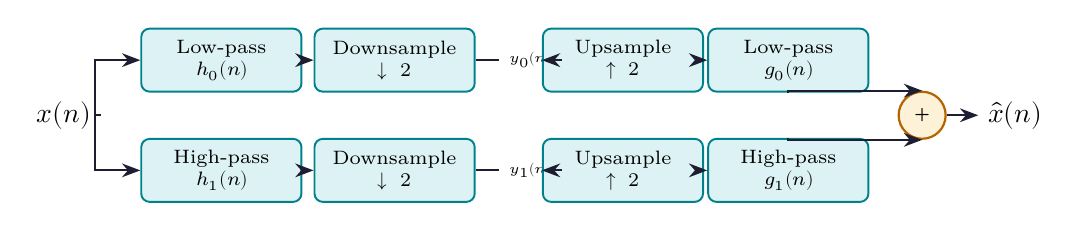
\begin{tikzpicture}[node distance=0.4cm and 0.8cm,
  sblock/.style={rectangle, draw=myteal, fill=hdrteal, text width=1.8cm,
    align=center, minimum height=0.8cm, font=\scriptsize,
    rounded corners=3pt, line width=0.7pt},
  junc/.style={circle, draw=myamber, fill=hdramber, minimum size=0.45cm,
    font=\tiny\bfseries, line width=0.8pt}]
    
  % Input
  \node (in) at (-0.5, 0) {$x(n)$};
  
  % Analysis Filters
  \node[sblock] (h0) at (1.5, 0.7) {Low-pass\\$h_0(n)$};
  \node[sblock] (h1) at (1.5, -0.7) {High-pass\\$h_1(n)$};
  \draw[arrow] (in) -- +(0.4, 0) |- (h0.west);
  \draw[arrow] (in) -- +(0.4, 0) |- (h1.west);
  
  % Downsamplers
  \node[sblock] (down0) at (3.7, 0.7) {Downsample\\$\downarrow 2$};
  \node[sblock] (down1) at (3.7, -0.7) {Downsample\\$\downarrow 2$};
  \draw[arrow] (h0) -- (down0);
  \draw[arrow] (h1) -- (down1);
  
  % Midpoints (subbands)
  \node (ch0) [right=0.3cm of down0] {\tiny $y_0(n)$};
  \node (ch1) [right=0.3cm of down1] {\tiny $y_1(n)$};
  \draw[line] (down0) -- (ch0);
  \draw[line] (down1) -- (ch1);

  % Upsamplers
  \node[sblock] (up0) at (6.6, 0.7) {Upsample\\$\uparrow 2$};
  \node[sblock] (up1) at (6.6, -0.7) {Upsample\\$\uparrow 2$};
  \draw[arrow] (ch0) -- (up0);
  \draw[arrow] (ch1) -- (up1);
  
  % Synthesis Filters
  \node[sblock] (g0) at (8.7, 0.7) {Low-pass\\$g_0(n)$};
  \node[sblock] (g1) at (8.7, -0.7) {High-pass\\$g_1(n)$};
  \draw[arrow] (up0) -- (g0);
  \draw[arrow] (up1) -- (g1);
  
  % Sum junction
  \node[junc] (sum) at (10.4, 0) {+};
  \draw[arrow] (g0) |- (sum.north);
  \draw[arrow] (g1) |- (sum.south);
  
  % Output
  \node (out) [right=0.4cm of sum] {$\hat{x}(n)$};
  \draw[arrow] (sum) -- (out);
\end{tikzpicture}
\end{tcolorbox}

\begin{itemize}[leftmargin=*, itemsep=3.5pt]
  \item \textbf{Analysis Bank:} Splits the signal into low-frequency approximation subband ($y_0$) and high-frequency detail subband ($y_1$). Downsampling ($\downarrow 2$) discards redundant odd samples.
  \item \textbf{Synthesis Bank:} Reconstructs the signal by upsampling ($\uparrow 2$, inserting zeros) and filtering.
  \item \textbf{Perfect Reconstruction Condition:} The filters must satisfy:
    \begin{align}
      g_0(n) &= h_0(-n), \quad g_1(n) = h_1(-n) \\
      H_0(-z)G_0(z) &+ H_1(-z)G_1(z) = 0 \quad \text{(Alias Cancellation)}
    \end{align}
  \item \textbf{Wavelet Packets:} In standard DWT, only the low-pass output is recursively decomposed. In \textbf{Wavelet Packet decomposition}, both the low-pass and high-pass branches are recursively filtered, producing a balanced tree.
\end{itemize}

% ===============================================================================
\section{Worked Examples}
% ===============================================================================

\begin{tcolorbox}[examplebox, title={1D Haar Wavelet Transform}]
\textbf{Problem:} Given a 4-point input signal $\mathbf{x} = [4, 6, 10, 12]^T$. Apply a 1-level Discrete Haar Wavelet Transform. Use the orthogonal Haar analysis filters:
\begin{align*}
  \text{Low-pass (approximation):} \quad h_0 &= \left[ \frac{1}{\sqrt{2}}, \frac{1}{\sqrt{2}} \right] \\[4pt]
  \text{High-pass (detail):} \quad h_1 &= \left[ \frac{1}{\sqrt{2}}, -\frac{1}{\sqrt{2}} \right]
\end{align*}
Compute the approximation coefficients $\mathbf{a}$ and detail coefficients $\mathbf{d}$ after downsampling.

\par\noindent\rule{\linewidth}{0.5pt}\par
\textbf{Solution:}
Discrete convolution is followed by downsampling by 2 ($\downarrow 2$). This is equivalent to applying the filters to non-overlapping pairs of input samples.

\textbf{1. Calculate Approximation Coefficients ($a_n$):}
\begin{itemize}[leftmargin=1.5em, itemsep=2.5pt]
  \item For the first pair $\{x(0), x(1)\} = \{4, 6\}$:
    \begin{equation*}
      a_0 = \frac{1}{\sqrt{2}}x(0) + \frac{1}{\sqrt{2}}x(1) = \frac{4 + 6}{\sqrt{2}} = \frac{10}{\sqrt{2}} = 5\sqrt{2} \approx 7.07
    \end{equation*}
  \item For the second pair $\{x(2), x(3)\} = \{10, 12\}$:
    \begin{equation*}
      a_1 = \frac{1}{\sqrt{2}}x(2) + \frac{1}{\sqrt{2}}x(3) = \frac{10 + 12}{\sqrt{2}} = \frac{22}{\sqrt{2}} = 11\sqrt{2} \approx 15.56
    \end{equation*}
\end{itemize}
So, the approximation coefficient vector is: $\mathbf{a} = [5\sqrt{2}, 11\sqrt{2}]^T$.

\textbf{2. Calculate Detail Coefficients ($d_n$):}
\begin{itemize}[leftmargin=1.5em, itemsep=2.5pt]
  \item For the first pair $\{4, 6\}$:
    \begin{equation*}
      d_0 = \frac{1}{\sqrt{2}}x(0) - \frac{1}{\sqrt{2}}x(1) = \frac{4 - 6}{\sqrt{2}} = \frac{-2}{\sqrt{2}} = -\sqrt{2} \approx -1.414
    \end{equation*}
  \item For the second pair $\{10, 12\}$:
    \begin{equation*}
      d_1 = \frac{1}{\sqrt{2}}x(2) - \frac{1}{\sqrt{2}}x(3) = \frac{10 - 12}{\sqrt{2}} = \frac{-2}{\sqrt{2}} = -\sqrt{2} \approx -1.414
    \end{equation*}
\end{itemize}
So, the detail coefficient vector is: $\mathbf{d} = [-\sqrt{2}, -\sqrt{2}]^T$.

\par\noindent\textbf{Final Haar Transform Output:}
The reconstructed representation is the combination of approximation and detail bands:
\begin{equation*}
  \mathbf{y} = [\mathbf{a} \mid \mathbf{d}]^T = [5\sqrt{2}, 11\sqrt{2}, -\sqrt{2}, -\sqrt{2}]^T
\end{equation*}
\end{tcolorbox}

\newpage

% ===============================================================================
% MANDATORY QUICK REVISION PAGE
% ===============================================================================
\begin{center}
  {\large\bfseries\color{myred} Quick Revision --- Module V}\\[3pt]
  {\small\color{mydark} Wavelets and Multi-resolution Image Processing $|$ PE-EC702B}
\end{center}
\noindent{\color{myred}\rule{\linewidth}{1.2pt}}
\vspace{4pt}

\begin{tcolorbox}[formulabox, title={\textbf{Key Formulas at a Glance}}]
\renewcommand{\arraystretch}{1.3}
\begin{tabularx}{\linewidth}{B{5.0cm} X}
Heisenberg Uncertainty & $\Delta t \cdot \Delta f \ge \frac{1}{4\pi}$ \\
Continuous Wavelet Transform & $W(a,b) = \int_{-\infty}^{\infty} f(t) \frac{1}{\sqrt{|a|}} \psi^*\left(\frac{t-b}{a}\right) \, dt$ \\
Scaling refinement eq. & $\phi(t) = \sqrt{2} \sum_n h_\phi(n) \phi(2t-n)$ \\
Wavelet refinement eq. & $\psi(t) = \sqrt{2} \sum_n h_\psi(n) \phi(2t-n)$ \\
Haar Scaling Coefficients & $h_\phi = \left[ \frac{1}{\sqrt{2}}, \frac{1}{\sqrt{2}} \right]$ \\
Haar Wavelet Coefficients & $h_\psi = \left[ \frac{1}{\sqrt{2}}, -\frac{1}{\sqrt{2}} \right]$
\end{tabularx}
\tcbset{colbacktitle=myteal, coltitle=white}
\end{tcolorbox}

\begin{tcolorbox}[defbox, title={\textbf{One-Line Definitions}}]
\begin{itemize}[leftmargin=*, itemsep=2.5pt, topsep=0pt]
  \item \textbf{Mother Wavelet:} A zero-mean, finite-energy prototype function $\psi(t)$ used to generate scaling bases.
  \item \textbf{MRA:} A mathematical framework that decomposes a signal into nested approximation spaces and details.
  \item \textbf{STFT:} A windowed Fourier transform that analyzes non-stationary signals using a fixed-width temporal slide.
  \item \textbf{Downsampling:} A process of discarding every alternate sample (e.g., $\downarrow 2$) to eliminate subband redundancy.
  \item \textbf{Wavelet Packets:} An expansion of DWT that decomposes both approximation and detail subbands recursively.
  \item \textbf{Admissibility Condition:} The zero-mean property required for wavelets to ensure the inverse transform exists.
\end{itemize}
\end{tcolorbox}

\begin{tcolorbox}[exambox, title={\textbf{Frequently Asked / Viva Questions}}]
\begin{enumerate}[leftmargin=*, itemsep=3.5pt, label=\arabic*.]
  \item \Q{Why is the standard Fourier Transform unsuitable for non-stationary signals?} Because it integrates over all time ($-\infty$ to $\infty$), meaning it yields spectral averages but completely loses the exact time locations of transient events.
  \item \Q{Explain the trade-off in STFT window sizing.} A wide window gives good frequency resolution but poor time resolution. A narrow window gives good time resolution but poor frequency resolution. It cannot adapt window width to frequency.
  \item \Q{How does the Wavelet Transform resolve the resolution trade-off in STFT?} It uses variable window sizes (multi-resolution): wide windows for low-frequency details (high frequency accuracy) and narrow windows for high-frequency details (high time accuracy).
  \item \Q{What are the physical roles of scaling and wavelet functions in MRA?} The scaling function $\phi(t)$ captures the low-frequency approximation of the signal, while the wavelet function $\psi(t)$ captures the high-frequency detail (edges).
  \item \Q{What is a 2-channel subband coder?} A system of filters and samplers that splits a signal into low-frequency (approximation) and high-frequency (detail) components, downsamples them, and later reconstructs them perfectly.
  \item \Q{State the perfect reconstruction (PR) condition for filter banks.} The analysis and synthesis filters must cancel aliasing caused by downsampling/upsampling ($H_0(-z)G_0(z) + H_1(-z)G_1(z) = 0$), and reconstruct the amplitude/phase without distortion.
  \item \Q{What is the difference between DWT and Wavelet Packet decomposition?} DWT decomposes only the low-pass approximation subband recursively at each level. Wavelet Packet decomposition decomposes both the low-pass and high-pass subbands recursively.
  \item \Q{State the properties of the Haar wavelet.} It is the oldest and simplest wavelet. It is discontinuous (step function), orthogonal, and has the shortest support (length 2), but has poor frequency selectivity.
  \item \Q{Why is downsampling necessary after subband filtering?} Because filtering halves the bandwidth of the signals. Downsampling by 2 eliminates the redundant samples, keeping the total number of samples constant.
  \item \Q{What is the scale parameter $a$ in CWT?} It represents scaling/stretching: small values of $a$ correspond to compressed wavelets (high frequencies), while large values of $a$ correspond to stretched wavelets (low frequencies).
\end{enumerate}
\tcbset{colbacktitle=myteal, coltitle=white}
\end{tcolorbox}

\begin{tcolorbox}[tikzbox, title={Fourier vs. STFT vs. Wavelet Transform}]
\centering
\renewcommand{\arraystretch}{1.2}
\begin{tabularx}{\linewidth}{>{\bfseries}B{3.2cm} Y Y Y}
\rowcolor{hdrgray} Feature & Fourier Transform & STFT & Wavelet Transform \\
\midrule
Time Resolution & None (infinite window) & Fixed (uniform window) & Variable (multi-resolution) \\
\rowcolor{rowalt} Window Width & Infinite & Fixed ($T$) & Decreases with frequency \\
Suitable For & Stationary signals & Quasi-stationary & Non-stationary (transients) \\
\bottomrule
\end{tabularx}
\tcbset{colbacktitle=myteal, coltitle=white}
\end{tcolorbox}


% -- Module 6 -----------------------------------------------------------------
\modulestart{6}{Redundancies in Digital Images}

\section{Redundancies in Digital Images}
% ===============================================================================

Data compression reduces the amount of data required to represent a given quantity of information by identifying and eliminating statistical redundancies.

\begin{tcolorbox}[defbox, title={Types of Image Redundancy}]
\begin{itemize}[leftmargin=*, itemsep=3.5pt]
  \item \textbf{Coding Redundancy:} Occurs when the codes assigned to gray levels do not minimize average code word length. Resolved by assigning shorter codes to highly probable intensities (entropy coding).
  \item \textbf{Inter-pixel (Spatial) Redundancy:} Results from the high correlation between adjacent pixels. We compress by encoding differences rather than absolute values (predictive coding).
  \item \textbf{Psycho-visual Redundancy:} Information that is ignored by the human visual system (e.g., fine details in highly textured or colored areas). Quantization represents this lossy elimination.
\end{itemize}
\end{tcolorbox}

% ===============================================================================
\section{Lossless Compression Methods}
% ===============================================================================

Lossless compression allows perfect reconstruction of the original image.

\subsection{Lossless Predictive Coding}
Based on eliminating inter-pixel redundancy. We predict the current pixel value $\hat{f}(n)$ based on past pixels, and encode the prediction error (residual):
\begin{equation}
  e(n) = f(n) - \text{round}\left[ \sum_{i=1}^m \alpha_i f(n-i) \right]
\end{equation}
The residual $e(n)$ has a highly peaked histogram centered at 0, which requires significantly fewer bits when entropy-coded.

\subsection{Entropy Coding}
\begin{itemize}[leftmargin=*, itemsep=3.5pt]
  \item \textbf{Huffman Coding:} A variable-length prefix coding technique. Assigns shorter binary codes to symbols with high probabilities, and longer codes to low probability ones.
  \item \textbf{Arithmetic Coding:} Maps the entire input symbol sequence into a single floating-point interval $[0,1)$. Highly efficient for skewed probability distributions.
  \item \textbf{LZW (Lempel-Ziv-Welch) Coding:} A dictionary-based algorithm. Replaces repeated sequences of symbols with indices from a dynamically generated dictionary. Used in GIF and TIFF formats.
\end{itemize}

% ===============================================================================
\section{Lossy Compression Methods}
% ===============================================================================

Lossy compression yields high compression ratios by discarding psycho-visually redundant information, preventing exact image reconstruction.

\subsection{Discrete Cosine Transform (DCT) and Transform Coding}
Transform coding maps pixels into the frequency domain, concentrating energy into a few coefficients. The 2D DCT is defined as:
\begin{equation}
  T(u,v) = \alpha(u)\alpha(v) \sum_{x=0}^{N-1} \sum_{y=0}^{N-1} f(x,y) \cos\left[ \frac{(2x+1)u\pi}{2N} \right] \cos\left[ \frac{(2y+1)v\pi}{2N} \right]
\end{equation}
where $N \times N$ is the subimage block size, and $\alpha(u) = \sqrt{1/N}$ for $u=0$, $\alpha(u) = \sqrt{2/N}$ for $u \neq 0$.
\par\noindent
The DCT has outstanding \textbf{energy compaction} (close to KLT) and avoids the blocking boundary discontinuities that DFT introduces.

% ===============================================================================
\section{Still Image Compression Standards}
% ===============================================================================

\subsection{JPEG Standard (DCT-Based)}
\begin{tcolorbox}[tikzbox, title={JPEG Encoder Block Diagram}]
\centering
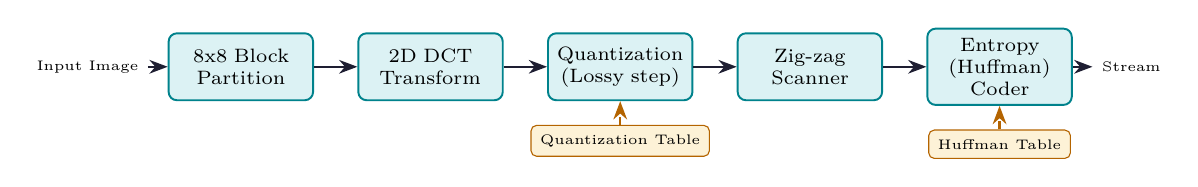
\begin{tikzpicture}[node distance=0.4cm and 0.55cm,
  sblock/.style={rectangle, draw=myteal, fill=hdrteal, text width=1.6cm,
    align=center, minimum height=0.85cm, font=\scriptsize,
    rounded corners=3pt, line width=0.7pt}]
    
  \node (in) at (-0.6, 0) {\tiny Input Image};
  \node[sblock, right=0.25cm of in] (part) {8x8 Block\\Partition};
  \node[sblock, right=of part] (dct) {2D DCT\\Transform};
  \node[sblock, right=of dct] (quant) {Quantization\\(Lossy step)};
  \node[sblock, right=of quant] (zig) {Zig-zag\\Scanner};
  \node[sblock, right=of zig] (ent) {Entropy\\(Huffman) Coder};
  \node (out) [right=0.25cm of ent] {\tiny Stream};
  
  \draw[arrow] (in) -- (part);
  \draw[arrow] (part) -- (dct);
  \draw[arrow] (dct) -- (quant);
  \draw[arrow] (quant) -- (zig);
  \draw[arrow] (zig) -- (ent);
  \draw[arrow] (ent) -- (out);
  
  \node[draw=myamber, fill=hdramber, rectangle, rounded corners=2pt, font=\tiny, below=0.3cm of quant] (qtbl) {Quantization Table};
  \draw[arrow, dashed, color=myamber] (qtbl) -- (quant);
  
  \node[draw=myamber, fill=hdramber, rectangle, rounded corners=2pt, font=\tiny, below=0.3cm of ent] (htbl) {Huffman Table};
  \draw[arrow, dashed, color=myamber] (htbl) -- (ent);
\end{tikzpicture}
\end{tcolorbox}

\begin{enumerate}[leftmargin=*, itemsep=3pt]
  \item \textbf{Image Partitioning:} Divide the image into non-overlapping $8 \times 8$ blocks.
  \item \textbf{DCT:} Apply 2D DCT to each block, producing 1 DC coefficient and 63 AC coefficients.
  \item \textbf{Quantization:} Divide each coefficient by its corresponding entry in a Quantization Table and round to the nearest integer. \textit{This is the only lossy step in JPEG.}
  \item \textbf{Zig-zag Scan:} Re-order the 2D matrix into a 1D vector in a zig-zag path, grouping low-frequency components together and producing long runs of zeros.
  \item \textbf{Entropy Coding:} Compress the values using Run-Length Coding (RLC) and Huffman coding.
\end{enumerate}

\subsection{JPEG-2000 Standard (DWT-Based)}
Instead of DCT, JPEG-2000 uses the \textbf{Discrete Wavelet Transform (DWT)}:
\begin{itemize}[leftmargin=*, itemsep=2.5pt]
  \item Eliminates the "blocking artifacts" visible in JPEG at high compression ratios.
  \item Employs EBCOT (Embedded Block Coding with Optimal Truncation).
  \item Supports progressive transmission (image loads from coarse to fine detail).
\end{itemize}

% ===============================================================================
\section{Worked Examples}
% ===============================================================================

\begin{tcolorbox}[examplebox, title={Huffman Coding Design}]
\textbf{Problem:} A discrete source emits 5 symbols with the following probabilities:
\begin{center}
  \small
  \begin{tabular}{c c c c c c}
    \toprule
    Symbol $s_i$ & $s_1$ & $s_2$ & $s_3$ & $s_4$ & $s_5$ \\
    \midrule
    Probability $P(s_i)$ & 0.4 & 0.2 & 0.2 & 0.1 & 0.1 \\
    \bottomrule
  \end{tabular}
\end{center}
\begin{enumerate}[label=(\alph*), leftmargin=*, itemsep=2pt]
  \item Construct the binary Huffman code for each symbol.
  \item Calculate the average code word length $L_{\text{avg}}$.
  \item Compute the source entropy $H(S)$.
  \item Calculate the coding efficiency $\eta$.
\end{enumerate}

\par\noindent\rule{\linewidth}{0.5pt}\par
\textbf{Solution:}

\textbf{(a) Code Word Construction:}
Combine the lowest probabilities recursively:
\begin{itemize}[leftmargin=1.5em, itemsep=2.5pt]
  \item Combine $s_4(0.1)$ and $s_5(0.1) \rightarrow s_{45}(0.2)$.
  \item Sort: $s_1(0.4)$, $s_2(0.2)$, $s_3(0.2)$, $s_{45}(0.2)$.
  \item Combine $s_3(0.2)$ and $s_{45}(0.2) \rightarrow s_{345}(0.4)$.
  \item Sort: $s_1(0.4)$, $s_{345}(0.4)$, $s_2(0.2)$.
  \item Combine $s_{345}(0.4)$ and $s_2(0.2) \rightarrow s_{2345}(0.6)$.
  \item Combine $s_1(0.4)$ and $s_{2345}(0.6) \rightarrow 1.0$.
\end{itemize}
Assigning bits (0 to upper, 1 to lower path):
\begin{itemize}[leftmargin=1.5em, itemsep=2pt]
  \item $s_1 \rightarrow 0$ (length 1)
  \item $s_2 \rightarrow 11$ (length 2)
  \item $s_3 \rightarrow 100$ (length 3)
  \item $s_4 \rightarrow 1010$ (length 4)
  \item $s_5 \rightarrow 1011$ (length 4)
\end{itemize}

\textbf{(b) Average Code Word Length ($L_{\text{avg}}$):}
\begin{equation*}
  L_{\text{avg}} = \sum P(s_i) l_i = 0.4(1) + 0.2(2) + 0.2(3) + 0.1(4) + 0.1(4) = 0.4 + 0.4 + 0.6 + 0.4 + 0.4 = 2.2 \text{ bits/sym}
\end{equation*}

\textbf{(c) Entropy ($H(S)$):}
\begin{align*}
  H(S) &= - \sum P(s_i) \log_2 P(s_i) \\
  &= - [0.4\log_2 0.4 + 2(0.2\log_2 0.2) + 2(0.1\log_2 0.1)] \\
  &= - [0.4(-1.322) + 0.4(-2.322) + 0.2(-3.322)] \\
  &= - [-0.529 - 0.929 - 0.664] = 2.122 \text{ bits/symbol}
\end{align*}

\textbf{(d) Coding Efficiency ($\eta$):}
\begin{equation*}
  \eta = \frac{H(S)}{L_{\text{avg}}} \times 100\% = \frac{2.122}{2.2} \times 100\% \approx 96.45\%
\end{equation*}
\end{tcolorbox}

\newpage

% ===============================================================================
% MANDATORY QUICK REVISION PAGE
% ===============================================================================
\begin{center}
  {\large\bfseries\color{myred} Quick Revision --- Module VI}\\[3pt]
  {\small\color{mydark} Image Compression $|$ PE-EC702B}
\end{center}
\noindent{\color{myred}\rule{\linewidth}{1.2pt}}
\vspace{4pt}

\begin{tcolorbox}[formulabox, title={\textbf{Key Formulas at a Glance}}]
\renewcommand{\arraystretch}{1.3}
\begin{tabularx}{\linewidth}{B{5.0cm} X}
Average Code Length & $L_{\text{avg}} = \sum_{i=1}^J P(s_i) l_i$ \\
Source Entropy & $H(S) = - \sum_{i=1}^J P(s_i) \log_2 P(s_i)$ \\
Coding Efficiency & $\eta = \frac{H(S)}{L_{\text{avg}}} \times 100\%$ \\
DPCM Residual Error & $e(n) = f(n) - \hat{f}(n)$ \\
2D Discrete Cosine Trans. & $T(u,v) = \alpha(u)\alpha(v) \sum_{x=0}^{N-1} \sum_{y=0}^{N-1} f(x,y) \cos\left[ \frac{(2x+1)u\pi}{2N} \right] \cos\left[ \frac{(2y+1)v\pi}{2N} \right]$ \\
Compression Ratio & $C_R = \frac{b_{\text{original}}}{b_{\text{compressed}}}$
\end{tabularx}
\tcbset{colbacktitle=myteal, coltitle=white}
\end{tcolorbox}

\begin{tcolorbox}[defbox, title={\textbf{One-Line Definitions}}]
\begin{itemize}[leftmargin=*, itemsep=2.5pt, topsep=0pt]
  \item \textbf{Coding Redundancy:} Redundancy occurring when code word lengths do not match the symbols' probability values.
  \item \textbf{Inter-pixel Redundancy:} Spatial correlation between neighboring pixels where values are highly predictable.
  \item \textbf{Psycho-visual Redundancy:} Visual details that can be eliminated without being noticed by human visual perception.
  \item \textbf{DPCM:} A predictive coding technique that encodes only the difference between actual and predicted pixel values.
  \item \textbf{Lossy Compression:} Compression that yields high ratios by discarding psycho-visual data, preventing exact recovery.
  \item \textbf{Zig-zag Scan:} A scan path in JPEG that orders 2D DCT coefficients to group zero values together for run-length coding.
\end{itemize}
\end{tcolorbox}

\begin{tcolorbox}[exambox, title={\textbf{Frequently Asked / Viva Questions}}]
\begin{enumerate}[leftmargin=*, itemsep=3.5pt, label=\arabic*.]
  \item \Q{What is the difference between lossless and lossy compression?} Lossless compression reconstructs the original image perfectly without any data loss. Lossy compression discards psycho-visual details to achieve much higher compression, but prevents perfect reconstruction.
  \item \Q{Which step in JPEG causes loss of information?} The Quantization step. Dividing the DCT coefficients by the quantization table values and rounding them to integers discards high-frequency details.
  \item \Q{What are blocking artifacts in JPEG?} At high compression ratios, the individual $8 \times 8$ blocks become visible in the reconstructed image as sharp grid discontinuities due to independent block processing.
  \item \Q{Why is DCT preferred over DFT for transform coding?} The DCT has better energy compaction properties and avoids the boundary discontinuities that the DFT introduces, reducing blocking artifacts.
  \item \Q{How does JPEG-2000 eliminate blocking artifacts?} It uses the Discrete Wavelet Transform (DWT) on the entire image (or large tiles) rather than the DCT on small $8 \times 8$ blocks.
  \item \Q{What is prefix code in Huffman coding?} A prefix code is a code in which no code word is a prefix of any other code word, ensuring that the code can be uniquely decoded in real-time.
  \item \Q{Define Shannon's First Source Coding Theorem.} It states that the minimum average code length required to represent a source without distortion is bounded below by the source entropy $H(S)$.
  \item \Q{Explain LZW coding.} It is a dictionary-based, lossless compression method that replaces recurring sequences of symbols with dictionary indices, commonly used in GIF files.
  \item \Q{What is the function of the zig-zag scan in JPEG?} It converts the 2D block of quantized coefficients into a 1D sequence, grouping high-frequency zero coefficients together to optimize Run-Length Encoding.
  \item \Q{How does Arithmetic Coding differ from Huffman Coding?} Huffman coding maps each individual symbol to a bit sequence. Arithmetic coding encodes the entire message as a single fractional value within an interval.
\end{enumerate}
\tcbset{colbacktitle=myteal, coltitle=white}
\end{tcolorbox}

\begin{tcolorbox}[tikzbox, title={JPEG vs. JPEG-2000 Comparison}]
\centering
\renewcommand{\arraystretch}{1.2}
\begin{tabularx}{\linewidth}{>{\bfseries}B{3.2cm} Y Y}
\rowcolor{hdrgray} Attribute & JPEG & JPEG-2000 \\
\midrule
Transform Method & Block-based 2D DCT ($8 \times 8$) & Full-image 2D DWT (Wavelet) \\
\rowcolor{rowalt} Compression artifacts & Blocking artifacts at high compression & Blurring / ringing at high compression \\
Progressive Display & Poor support & High support (resolution scalability) \\
\bottomrule
\end{tabularx}
\tcbset{colbacktitle=myteal, coltitle=white}
\end{tcolorbox}


% -- Module 7 -----------------------------------------------------------------
\modulestart{7}{Inter-Frame Redundancy}

\section{Inter-Frame Redundancy}
% ===============================================================================

A video sequence is a series of consecutive images (frames) captured over time.

\begin{tcolorbox}[defbox, title={Temporal Redundancy}]
\textbf{Inter-Frame (Temporal) Redundancy:} Refers to the massive statistical correlation between successive frames. Since video frames are captured at high rates (typically 24 to 60 frames/sec), adjacent frames contain nearly identical background and object structures, with only minor spatial displacements.
\end{tcolorbox}

% ===============================================================================
\section{Motion Estimation and Compensation}
% ===============================================================================

Motion estimation detects displacements of objects between frames, while motion compensation encodes only the difference (prediction residual) and the motion displacement vectors.

\subsection{Block Matching Algorithm (BMA)}
The standard method for motion estimation.
\begin{itemize}[leftmargin=*, itemsep=3pt]
  \item The current frame is divided into non-overlapping macroblocks of size $N \times N$ (typically $16 \times 16$).
  \item For each block, we search for the best matching block in a reference frame (past or future) within a search range $[-p, p]$.
  \item \textbf{Search Metrics:} Used to measure block similarity. The most common is the \textbf{Mean Absolute Difference (MAD)}:
    \begin{equation}
      \text{MAD}(i,j) = \frac{1}{N^2} \sum_{x=0}^{N-1} \sum_{y=0}^{N-1} \left| F_t(x,y) - F_{t-1}(x+i, y+j) \right|
    \end{equation}
    where $F_t$ is the current block and $F_{t-1}$ is the reference block shifted by displacement $(i,j)$ (Motion Vector).
\end{itemize}

\subsection{Search Strategies}
\begin{itemize}[leftmargin=*, itemsep=3.5pt]
  \item \textbf{Full Search (Exhaustive Search):} Evaluates MAD at every possible integer pixel shift within $[-p, p]$. Guarantees finding the global minimum, but is computationally extremely heavy.
  \item \textbf{Three-Step Search (TSS):} A fast, logarithmic search strategy:
    \begin{enumerate}[label=\alph*., leftmargin=1.5em, itemsep=1.5pt]
      \item Start at center, evaluate 9 search locations with a coarse step size $S = \lfloor p/2 \rfloor$.
      \item Move center to the location yielding minimum MAD. Reduce step size to $S = S/2$.
      \item Evaluate 8 new locations around the new center. Repeat until step size is $1$.
    \end{enumerate}
    \textit{Computational savings: Requires only 25 computations for $p=7$, compared to 225 for Full Search.}
\end{itemize}

% ===============================================================================
\section{Frame Classification and Sequence Hierarchy}
% ===============================================================================

Video coding standards classify frames into three types to optimize prediction efficiency:
\begin{itemize}[leftmargin=*, itemsep=3.5pt]
  \item \textbf{I-Frames (Intra-Coded):} Coded independently of other frames using still-image compression (like JPEG). Acts as random access points. Low compression.
  \item \textbf{P-Frames (Predicted):} Coded using forward motion prediction from a previous reference frame (I or P). Moderate compression.
  \item \textbf{B-Frames (Bidirectional Predictive):} Coded using both past and future reference frames (forward and backward prediction). Yields the highest compression ratios.
\end{itemize}

\begin{tcolorbox}[defbox, title={Video Sequence Structure}]
\textbf{Group of Pictures (GOP):} The sequence structure of I, P, and B frames. A typical GOP pattern is:
\begin{center}
  \textbf{I\quad B\quad B\quad P\quad B\quad B\quad P\quad B\quad B\quad I}
\end{center}
\par\noindent
\textbf{Hierarchy:} Video Session $\rightarrow$ GOP $\rightarrow$ Picture/Frame $\rightarrow$ Slices $\rightarrow$ Macroblocks ($16\times16$) $\rightarrow$ Blocks ($8\times8$).
\end{tcolorbox}

% ===============================================================================
\section{Hybrid Video Encoder and Standards}
% ===============================================================================

Modern video compression standards use a hybrid framework combining DPCM predictive loop (motion estimation) with spatial transform coding (2D DCT).

\begin{tcolorbox}[tikzbox, title={Hybrid Video Encoder Block Diagram}]
\centering
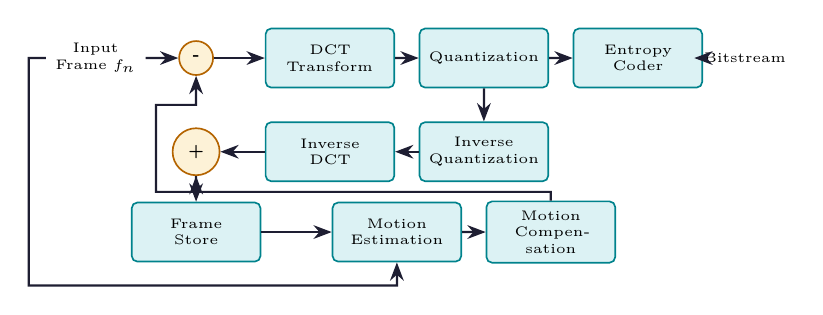
\begin{tikzpicture}[scale=0.85, every node/.style={font=\tiny}]
  \tikzset{
    sblock/.style={rectangle, draw=myteal, fill=hdrteal, text width=1.4cm,
      align=center, minimum height=0.75cm, font=\tiny,
      rounded corners=2pt, line width=0.6pt},
    junc/.style={circle, draw=myamber, fill=hdramber, minimum size=0.4cm,
      font=\tiny\bfseries, line width=0.6pt}
  }
  
  % Input frame
  \node (in) at (-1, 1.2) [align=center] {Input\\Frame $f_n$};
  
  % Sum junction to subtract prediction
  \node[junc] (diff) at (0.5, 1.2) {-};
  \draw[arrow] (in) -- (diff);
  
  % DCT
  \node[sblock] (dct) at (2.5, 1.2) {DCT\\Transform};
  \draw[arrow] (diff) -- (dct);
  
  % Quantization
  \node[sblock] (quant) at (4.8, 1.2) {Quantization};
  \draw[arrow] (dct) -- (quant);
  
  % Entropy Coder
  \node[sblock] (ent) at (7.1, 1.2) {Entropy\\Coder};
  \draw[arrow] (quant) -- (ent);
  
  % Output
  \node (out) at (8.7, 1.2) {Bitstream};
  \draw[arrow] (ent) -- (out);
  
  % Inverse Quantization
  \node[sblock] (iquant) at (4.8, -0.2) {Inverse\\Quantization};
  \draw[arrow] (quant) -- (iquant);
  
  % Inverse DCT
  \node[sblock] (idct) at (2.5, -0.2) {Inverse\\DCT};
  \draw[arrow] (iquant) -- (idct);
  
  % Reconstruction Summer
  \node[junc] (recon) at (0.5, -0.2) {+};
  \draw[arrow] (idct) -- (recon);
  
  % Frame Store
  \node[sblock] (store) at (0.5, -1.4) {Frame\\Store};
  \draw[arrow] (recon) -- (store);
  
  % Motion Estimation
  \node[sblock] (me) at (3.5, -1.4) {Motion\\Estimation};
  \draw[arrow] (store) -- (me);
  
  % Motion Compensation
  \node[sblock] (mc) at (5.8, -1.4) {Motion\\Compensation};
  \draw[arrow] (me) -- (mc);
  
  % Connections from Motion Compensation back to diff and recon
  \draw[arrow] (mc.north) |- (0.5, -0.8) -- (recon.south);
  \draw[arrow] (0.5, -0.8) -- (-0.1, -0.8) |- (0.5, 0.5) -- (diff.south);
  
  % Connection from Input frame to Motion Estimation
  \draw[arrow] (in.west) -- (-2.0, 1.2) |- (3.5, -2.2) -- (me.south);
\end{tikzpicture}
\end{tcolorbox}

\subsection{Video Standards}
\begin{itemize}[leftmargin=*, itemsep=3.5pt]
  \item \textbf{MPEG-1 / MPEG-2:} Formats used for VCDs ($MPEG-1$) and DVDs/Digital TV ($MPEG-2$).
  \item \textbf{H.264/AVC:} Incorporates intra-frame spatial prediction, quarter-pixel motion vector accuracy, and variable block sizes ($16\times16$ down to $4\times4$).
  \item \textbf{H.265/HEVC:} Replaces macroblocks with Coding Tree Units (CTUs) of size up to $64\times64$, reducing bitrates by $50\%$ compared to H.264 for equivalent quality.
\end{itemize}

% ===============================================================================
\section{Worked Examples}
% ===============================================================================

\begin{tcolorbox}[examplebox, title={Motion Vector Estimation}]
\textbf{Problem:} Given a $2 \times 2$ macroblock in the current frame $F_t$ and its corresponding search region in the reference frame $F_{t-1}$. Calculate the Mean Absolute Difference (MAD) for candidate displacement vectors $\mathbf{v}_1 = (0,0)$ and $\mathbf{v}_2 = (0,1)$, and identify the optimal motion vector.

\par\vspace{6pt}\noindent
\begin{minipage}{0.42\textwidth}
  \centering
  \textbf{Current Block $F_t$:}
  \[
    F_t = \begin{bmatrix} 80 & 85 \\ 70 & 75 \end{bmatrix}
  \]
\end{minipage}
\hfill
\begin{minipage}{0.53\textwidth}
  \centering
  \textbf{Reference Search Region $F_{t-1}$:}
  \par\vspace{4pt}
  \small
  \begin{tabular}{c | c c c}
    & $x=-1$ & $x=0$ & $x=1$ \\
    \hline
    $y=-1$ & 78 & 82 & 88 \\
    $y=0$  & 72 & \textbf{80} & \textbf{84} \\
    $y=1$  & 65 & \textbf{71} & \textbf{76}
  \end{tabular}
\end{minipage}
\par\vspace{6pt}

\par\noindent\rule{\linewidth}{0.5pt}\par
\textbf{Solution:}

\textbf{(a) For $\mathbf{v}_1 = (0,0)$:}
The candidate block in $F_{t-1}$ starting at $(0,0)$ is:
\[
  \begin{bmatrix} 80 & 84 \\ 71 & 76 \end{bmatrix}
\]
Compute the absolute differences:
\begin{align*}
  \text{Diff} &= \begin{bmatrix} |80 - 80| & |85 - 84| \\ |70 - 71| & |75 - 76| \end{bmatrix} = \begin{bmatrix} 0 & 1 \\ 1 & 1 \end{bmatrix} \\
  \text{MAD}(0,0) &= \frac{0 + 1 + 1 + 1}{4} = \frac{3}{4} = 0.75
\end{align*}

\textbf{(b) For $\mathbf{v}_2 = (0,1)$ (vertical shift by $j=1$):}
The candidate block in $F_{t-1}$ shifted by $(0,1)$ is:
\[
  \begin{bmatrix} F_{t-1}(0,1) & F_{t-1}(1,1) \\ F_{t-1}(0,2) & F_{t-1}(1,2) \end{bmatrix} = \begin{bmatrix} 71 & 76 \\ \text{N/A} & \text{N/A} \end{bmatrix}
\]
Since this candidate block contains out-of-bounds elements ($\text{N/A}$), we cannot calculate a valid MAD for $\mathbf{v}_2 = (0,1)$.

\par\vspace{6pt}
\textbf{Alternative Candidate Analysis:}
Let us analyze displacement $(i,j) = (-1,-1)$ (shifted top-left by 1 pixel) as an alternative candidate:
\begin{itemize}[leftmargin=*, itemsep=4pt]
  \item The candidate block in $F_{t-1}$ for $(i,j) = (-1,-1)$ is:
    \[
      \begin{bmatrix} F_{t-1}(-1,-1) & F_{t-1}(0,-1) \\ F_{t-1}(-1,0) & F_{t-1}(0,0) \end{bmatrix} = \begin{bmatrix} 78 & 82 \\ 72 & 80 \end{bmatrix}
    \]
  \item Compute the absolute differences with the current block $F_t$:
    \[
      \text{Diff} = \begin{bmatrix} |80 - 78| & |85 - 82| \\ |70 - 72| & |75 - 80| \end{bmatrix} = \begin{bmatrix} 2 & 3 \\ 2 & 5 \end{bmatrix}
    \]
  \item Calculate the MAD:
    \[
      \text{MAD}(-1,-1) = \frac{2 + 3 + 2 + 5}{4} = \frac{12}{4} = 3.00
    \]
\end{itemize}

\par\vspace{6pt}
\textbf{Conclusion and Motion Vector Selection:}
Comparing the calculated MAD values:
\begin{itemize}[leftmargin=*, itemsep=3pt]
  \item $\text{MAD}(0,0) = 0.75$
  \item $\text{MAD}(-1,-1) = 3.00$
\end{itemize}
Since $\text{MAD}(0,0) < \text{MAD}(-1,-1)$, the motion vector $\mathbf{v} = (0,0)$ is selected as the preferred motion vector.
\end{tcolorbox}

\newpage

% ===============================================================================
% MANDATORY QUICK REVISION PAGE
% ===============================================================================
\begin{center}
  {\large\bfseries\color{myred} Quick Revision --- Module VII}\\[3pt]
  {\small\color{mydark} Fundamentals of Video Coding $|$ PE-EC702B}
\end{center}
\noindent{\color{myred}\rule{\linewidth}{1.2pt}}
\vspace{4pt}

\begin{tcolorbox}[formulabox, title={\textbf{Key Formulas at a Glance}}]
\renewcommand{\arraystretch}{1.3}
\begin{tabularx}{\linewidth}{B{5.0cm} X}
Mean Absolute Difference & $\text{MAD}(i,j) = \frac{1}{N^2} \sum_{x=0}^{N-1} \sum_{y=0}^{N-1} \left| F_t(x,y) - F_{t-1}(x+i, y+j) \right|$ \\
Mean Squared Error & $\text{MSE}(i,j) = \frac{1}{N^2} \sum_{x=0}^{N-1} \sum_{y=0}^{N-1} \left[ F_t(x,y) - F_{t-1}(x+i, y+j) \right]^2$ \\
Search Complexity (Full) & $N_{\text{eval}} = (2p + 1)^2$ \quad ($p$ = search range) \\
Search Complexity (TSS) & $N_{\text{eval}} \approx 9 + 8 \log_2(p)$ \\
Motion Compensation Error & $e_t(x,y) = F_t(x,y) - F_{t-1}(x + dx, y + dy)$
\end{tabularx}
\tcbset{colbacktitle=myteal, coltitle=white}
\end{tcolorbox}

\begin{tcolorbox}[defbox, title={\textbf{One-Line Definitions}}]
\begin{itemize}[leftmargin=*, itemsep=2.5pt, topsep=0pt]
  \item \textbf{Motion Estimation:} The process of locating the displacement vector of a macroblock between successive video frames.
  \item \textbf{Motion Compensation:} The process of reconstructing a frame by shifting reference frame pixels using motion vectors.
  \item \textbf{I-Frame:} An intra-coded frame compressed independently using spatial details, acting as a random access sync point.
  \item \textbf{P-Frame:} A predicted frame coded using forward temporal prediction from a single preceding reference frame.
  \item \textbf{B-Frame:} A bidirectional frame coded using both past and future reference frames, offering maximum compression.
  \item \textbf{GOP:} Group of Pictures, defining the recurring sequence pattern of I, P, and B frames in a video stream.
\end{itemize}
\end{tcolorbox}

\begin{tcolorbox}[exambox, title={\textbf{Frequently Asked / Viva Questions}}]
\begin{enumerate}[leftmargin=*, itemsep=3.5pt, label=\arabic*.]
  \item \Q{What is temporal redundancy in video coding?} It is the high correlation between consecutive frames in a video sequence, where background and moving objects remain mostly identical from frame to frame.
  \item \Q{How does the Hybrid Video Encoder combine spatial and temporal compression?} It uses motion estimation (temporal prediction) to generate a residual prediction error, which is then compressed using 2D DCT and quantization (spatial transform coding).
  \item \Q{Why do B-frames achieve much higher compression than P-frames?} Because B-frames use bidirectional prediction, meaning they can reference macroblocks from both past and future frames, yielding smaller prediction errors.
  \item \Q{What is the trade-off of using a large number of B-frames in video streaming?} B-frames require future frames to be decoded first, which introduces frame buffering delay (latency) and increases decoder memory requirements.
  \item \Q{Explain the Three-Step Search (TSS) algorithm.} It is a fast search method that evaluates 9 points using a coarse step size, shifts the center to the minimum error point, halves the step size, and repeats until the step size is 1.
  \item \Q{What is a macroblock in video standards?} A macroblock is a $16 \times 16$ pixel region of luminance (Y) along with the corresponding chrominance (U, V) blocks, representing the basic processing unit for motion compensation.
  \item \Q{State the main advantage of H.264/AVC over MPEG-2.} H.264/AVC achieves comparable visual quality at approximately half the bitrate of MPEG-2 by using intra-prediction, multi-frame references, and variable block sizes.
  \item \Q{What are CTUs in H.265/HEVC?} Coding Tree Units (CTUs) replace macroblocks in H.265. They can be dynamically partitioned into Coding Units (CUs) from $64 \times 64$ down to $8 \times 8$, optimizing compression for high-resolution (4K/8K) video.
  \item \Q{Why are P-frames and B-frames unsuitable as random access entry points?} Because they contain temporal prediction residuals, meaning they cannot be decoded without first decoding their past and future reference frames.
  \item \Q{Define the Motion Vector.} The displacement vector $(dx, dy)$ representing the horizontal and vertical offset of a matching block in the reference frame relative to the current frame.
\end{enumerate}
\tcbset{colbacktitle=myteal, coltitle=white}
\end{tcolorbox}

\begin{tcolorbox}[tikzbox, title={Comparison of Video Frame Types}]
\centering
\renewcommand{\arraystretch}{1.2}
\begin{tabularx}{\linewidth}{>{\bfseries}B{3.2cm} Y Y Y}
\rowcolor{hdrgray} Attribute & I-Frame (Intra) & P-Frame (Predicted) & B-Frame (Bidirectional) \\
\midrule
Coding Source & Self-contained (spatial) & Temporal (forward) & Temporal (bidirectional) \\
\rowcolor{rowalt} Compression Ratio & Low ($2:1$ to $5:1$) & Moderate ($10:1$ to $20:1$) & High ($30:1$ to $50:1$) \\
Random Access Point & Yes & No & No \\
\bottomrule
\end{tabularx}
\tcbset{colbacktitle=myteal, coltitle=white}
\end{tcolorbox}


% -- Module 8 -----------------------------------------------------------------
\modulestart{8}{Temporal Video Segmentation}

\section{Temporal Video Segmentation}
% ===============================================================================

Video segmentation partitions a video sequence into structurally meaningful units. Temporal segmentation focuses on dividing the video stream into continuous camera sequences called \textbf{shots}.

\begin{tcolorbox}[defbox, title={Video Shot Definitions}]
\textbf{Video Shot:} A continuous sequence of frames captured by a single camera without interruption.
\par\noindent
\textbf{Shot Boundary:} The transition point between two consecutive shots. These are classified into:
\begin{itemize}[leftmargin=*, itemsep=1.5pt]
  \item \textbf{Hard-Cuts (Abrupt):} Instantaneous transition occurring between two adjacent frames (frame $t$ is from camera A, frame $t+1$ is from camera B).
  \item \textbf{Soft-Cuts (Gradual):} Dispersed transitions taking place over multiple frames (e.g., fades, dissolves, wipes).
\end{itemize}
\end{tcolorbox}

\begin{tcolorbox}[tikzbox, title={Shot Boundary Transition Tree}]
\centering
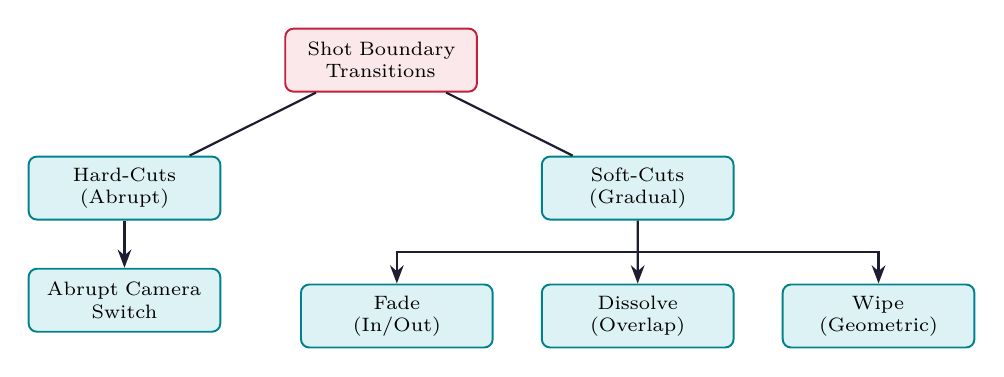
\begin{tikzpicture}[node distance=0.8cm and 0.6cm,
  sblock/.style={rectangle, draw=myteal, fill=hdrteal, text width=2.2cm,
    align=center, minimum height=0.8cm, font=\scriptsize,
    rounded corners=3pt, line width=0.7pt}]
    
  \node[sblock, draw=myred, fill=hdrred] (root) {Shot Boundary\\Transitions};
  
  \node[sblock, below left=0.8cm and 0.8cm of root] (hard) {Hard-Cuts\\(Abrupt)};
  \node[sblock, below right=0.8cm and 0.8cm of root] (soft) {Soft-Cuts\\(Gradual)};
  
  \draw[line] (root) -- (hard);
  \draw[line] (root) -- (soft);
  
  \node[sblock, below=0.6cm of hard] (cut) {Abrupt Camera\\Switch};
  \draw[arrow] (hard) -- (cut);
  
  \node[sblock, below=0.8cm of soft] (dissolve) {Dissolve\\(Overlap)};
  \node[sblock, left=0.6cm of dissolve] (fade) {Fade\\(In/Out)};
  \node[sblock, right=0.6cm of dissolve] (wipe) {Wipe\\(Geometric)};
  
  \draw[line] (soft.south) -- ($(soft.south)!0.5!(dissolve.north)$) coordinate (branch);
  \draw[arrow] (branch) -- (dissolve.north);
  \draw[arrow] (branch) -| (fade.north);
  \draw[arrow] (branch) -| (wipe.north);
\end{tikzpicture}
\end{tcolorbox}

\subsection{Detection Algorithms}
\begin{enumerate}[leftmargin=*, itemsep=3.5pt]
  \item \textbf{Pixel-Level Differencing:} Measures the average intensity change between pixels:
    \begin{equation}
      D(t, t-1) = \frac{1}{MN} \sum_{x=0}^{M-1} \sum_{y=0}^{N-1} \left| f_t(x,y) - f_{t-1}(x,y) \right|
    \end{equation}
    Highly sensitive to object and camera motion.
  \item \textbf{Histogram-Level Differencing:} Compares the intensity histograms of adjacent frames:
    \begin{equation}
      D_H(t, t-1) = \sum_{k=0}^{L-1} \left| h_t(k) - h_{t-1}(k) \right|
    \end{equation}
    Robust against minor object movements and camera pans.
  \item \textbf{Edge Change Ratio (ECR):} Measures the entry and exit of edge pixels between frames, highly effective at detecting soft-cuts.
\end{enumerate}

% ===============================================================================
\section{Spatial/Motion-Based Segmentation}
% ===============================================================================

Spatial segmentation separates moving foreground objects from static backgrounds.

\begin{itemize}[leftmargin=*, itemsep=3.5pt]
  \item \textbf{Background Subtraction:} Thresholds the difference between the current frame $f_t(x,y)$ and a reference background model $B(x,y)$:
    \begin{equation}
      |f_t(x,y) - B(x,y)| > T
    \end{equation}
    The background $B(x,y)$ is updated recursively (e.g., using Mixture of Gaussians).
  \item \textbf{Temporal Differencing:} Detects motion by subtracting adjacent frames:
    \begin{equation}
      |f_t(x,y) - f_{t-1}(x,y)| > T
    \end{equation}
    More adaptive to dynamic backgrounds, but fails to segment the interior of uniformly colored moving objects (the "ghosting" effect).
  \item \textbf{Optical Flow:} Computes the 2D velocity vector field representing the apparent motion of pixels. Highly complex, but provides detailed motion direction.
\end{itemize}

% ===============================================================================
\section{Video Object Detection and Tracking}
% ===============================================================================

Object tracking monitors the position and trajectory of a segmented object over time.

\begin{enumerate}[leftmargin=*, itemsep=3.5pt]
  \item \textbf{Kalman Filter:} A recursive estimator that predicts the state (position, velocity) of a moving object and corrects the prediction using noisy measurements. Operates in two steps:
    \begin{itemize}[leftmargin=1em, itemsep=1.5pt]
      \item \textit{Predict:} Project the state ahead: $\hat{\mathbf{x}}_k^- = \mathbf{A}\hat{\mathbf{x}}_{k-1}$.
      \item \textit{Correct:} Update the estimate using the measurement: $\hat{\mathbf{x}}_k = \hat{\mathbf{x}}_k^- + \mathbf{K}_k(\mathbf{z}_k - \mathbf{H}\hat{\mathbf{x}}_k^-)$.
    \end{itemize}
  \item \textbf{Mean-Shift Tracking:} A non-parametric iterative algorithm that locates the local maxima (peak) of a probability distribution (e.g., color histogram). It moves a tracking window towards the center of gravity of the target color distribution in each frame.
  \item \textbf{Particle Filters:} Uses Monte Carlo simulations (representing the target state probability distribution by a set of weighted particles) to track objects in non-Gaussian, non-linear environments.
\end{enumerate}

% ===============================================================================
\section{Worked Examples}
% ===============================================================================

\begin{tcolorbox}[examplebox, title={Temporal Differencing and Boundary Detection}]
\textbf{Problem:} Given two simplified $3 \times 3$ matrices representing consecutive video frames $F_{t-1}$ and $F_t$:
\begin{center}
  $F_{t-1} = \begin{bmatrix} 50 & 52 & 50 \\ 48 & 50 & 52 \\ 50 & 48 & 50 \end{bmatrix}, \quad
  F_t = \begin{bmatrix} 70 & 75 & 70 \\ 68 & 72 & 75 \\ 70 & 68 & 70 \end{bmatrix}$
\end{center}
\begin{enumerate}[label=(\alph*), leftmargin=*, itemsep=2.5pt]
  \item Calculate the pixel-level average difference metric $D(t, t-1)$.
  \item Given a threshold $T_{\text{cut}} = 15$, determine if a shot boundary transition is detected between these two frames.
\end{enumerate}

\par\noindent\rule{\linewidth}{0.5pt}\par
\textbf{Solution:}

\textbf{(a) Average Difference Calculation ($D(t, t-1)$):}
Subtract the matrices element-by-element and take the absolute values:
\begin{align*}
  |F_t - F_{t-1}| &= \begin{bmatrix} |70 - 50| & |75 - 52| & |70 - 50| \\ |68 - 48| & |72 - 50| & |75 - 52| \\ |70 - 50| & |68 - 48| & |70 - 50| \end{bmatrix} \\
  &= \begin{bmatrix} 20 & 23 & 20 \\ 20 & 22 & 23 \\ 20 & 20 & 20 \end{bmatrix}
\end{align*}
Now, compute the average over the 9 pixels ($MN = 9$):
\begin{equation*}
  D(t, t-1) = \frac{20 + 23 + 20 + 20 + 22 + 23 + 20 + 20 + 20}{9} = \frac{188}{9} \approx 20.89
\end{equation*}

\textbf{(b) Shot Boundary Decision:}
\begin{itemize}[leftmargin=*, itemsep=2pt]
  \item The computed average difference metric $D(t, t-1) = 20.89$.
  \item The boundary threshold $T_{\text{cut}} = 15$.
  \item Since $D(t, t-1) = 20.89 > T_{\text{cut}} = 15$, a shot boundary transition is indeed detected between frame $t-1$ and frame $t$.
\end{itemize}
\end{tcolorbox}

\newpage

% ===============================================================================
% MANDATORY QUICK REVISION PAGE
% ===============================================================================
\begin{center}
  {\large\bfseries\color{myred} Quick Revision --- Module VIII}\\[3pt]
  {\small\color{mydark} Video Segmentation $|$ PE-EC702B}
\end{center}
\noindent{\color{myred}\rule{\linewidth}{1.2pt}}
\vspace{4pt}

\begin{tcolorbox}[formulabox, title={\textbf{Key Formulas at a Glance}}]
\renewcommand{\arraystretch}{1.3}
\begin{tabularx}{\linewidth}{B{5.0cm} X}
Pixel Difference Metric & $D(t, t-1) = \frac{1}{MN} \sum_{x=0}^{M-1} \sum_{y=0}^{N-1} \left| f_t(x,y) - f_{t-1}(x,y) \right|$ \\
Histogram Difference & $D_H(t, t-1) = \sum_{k=0}^{L-1} \left| h_t(k) - h_{t-1}(k) \right|$ \\
Background Subtraction & $|f_t(x,y) - B(x,y)| > T$ \\
Temporal Differencing & $|f_t(x,y) - f_{t-1}(x,y)| > T$ \\
Kalman State Prediction & $\hat{\mathbf{x}}_k^- = \mathbf{A}\hat{\mathbf{x}}_{k-1}$ \\
Kalman Measurement Update & $\hat{\mathbf{x}}_k = \hat{\mathbf{x}}_k^- + \mathbf{K}_k(\mathbf{z}_k - \mathbf{H}\hat{\mathbf{x}}_k^-)$
\end{tabularx}
\tcbset{colbacktitle=myteal, coltitle=white}
\end{tcolorbox}

\begin{tcolorbox}[defbox, title={\textbf{One-Line Definitions}}]
\begin{itemize}[leftmargin=*, itemsep=2.5pt, topsep=0pt]
  \item \textbf{Hard-Cut:} An abrupt change between two consecutive frames due to camera switching, marking a shot boundary.
  \item \textbf{Soft-Cut:} A gradual, multi-frame transition (such as fade, dissolve, or wipe) between two video shots.
  \item \textbf{Background Subtraction:} A spatial differencing technique that isolates foreground objects by subtracting a background model.
  \item \textbf{Temporal Differencing:} Isolating motion by thresholding the difference between consecutive video frames.
  \item \textbf{Mean-Shift:} An iterative peak-search algorithm that tracks target centers by maximizing color probability distributions.
  \item \textbf{Optical Flow:} A vector field representing the apparent velocity of moving pixels across consecutive frames.
\end{itemize}
\end{tcolorbox}

\begin{tcolorbox}[exambox, title={\textbf{Frequently Asked / Viva Questions}}]
\begin{enumerate}[leftmargin=*, itemsep=3.5pt, label=\arabic*.]
  \item \Q{What is the difference between a hard-cut and a soft-cut transition?} A hard-cut is an abrupt, instantaneous shot transition occurring between two adjacent frames. A soft-cut is a gradual transition (such as a fade, dissolve, or wipe) that spans multiple frames.
  \item \Q{Why is histogram-level differencing preferred over pixel-level differencing for shot boundary detection?} Pixel-level differencing is highly sensitive to camera panning, zoom, and local object motion. Histogram-level differencing is robust to these changes since the overall color distribution remains similar.
  \item \Q{Explain the ghosting effect in temporal differencing.} If a moving object has a uniform interior color, subtracting adjacent frames yields differences only at the leading and trailing edges, leaving the interior segmented as background (hollow "ghost" region).
  \item \Q{How does Background Subtraction model dynamic elements like swaying trees?} By recursively updating the background model using a mixture of Gaussians (MoG) that models multiple intensity distributions for each pixel location.
  \item \Q{State the two phases of the Kalman Filter.} (1) The Prediction phase (projects the current state and error covariance estimate forward in time), and (2) the Correction/Measurement update phase (adjusts the estimate using the new sensor measurement).
  \item \Q{What is the role of the Kalman Gain $K_k$?} The Kalman gain decides the weighting between the predicted state estimate and the new measurement. If measurement noise is low, $K_k$ weights the measurement heavily; if high, it weights the prediction.
  \item \Q{Explain the difference between object detection and object tracking.} Object detection identifies and locates objects of interest in individual frames. Object tracking links these detections across consecutive frames to trace the object's path.
  \item \Q{How does the Mean-Shift algorithm track a target?} It iteratively computes the mean shift vector (displacement between the current window center and the color distribution's center of gravity) and shifts the window until convergence.
  \item \Q{What are the types of gradual transitions (soft-cuts) in video?} (1) Fade-in/out (gradual change from/to a solid black frame), (2) Dissolve (one scene overlaps and replaces another gradually), and (3) Wipe (a geometric line sweeps across the screen).
  \item \Q{What is the limitation of optical flow estimation?} Optical flow is computationally extremely intensive, making it difficult to implement in real-time without specialized hardware, and it is sensitive to illumination changes.
\end{enumerate}
\tcbset{colbacktitle=myteal, coltitle=white}
\end{tcolorbox}

\begin{tcolorbox}[tikzbox, title={Hard-Cut vs. Soft-Cut Shot Boundaries}]
\centering
\renewcommand{\arraystretch}{1.2}
\begin{tabularx}{\linewidth}{>{\bfseries}B{3.2cm} Y Y}
\rowcolor{hdrgray} Attribute & Hard-Cut Transition & Soft-Cut (Gradual) Transition \\
\midrule
Duration & Exactly 1 frame boundary & Spans multiple frames (typically 10-30) \\
\rowcolor{rowalt} Visual transition & Abrupt camera scene switch & Smooth fade, overlap (dissolve), or sweep (wipe) \\
Detection Metric & High spike in frame differences & Broad, low-amplitude peak in differences \\
\bottomrule
\end{tabularx}
\tcbset{colbacktitle=myteal, coltitle=white}
\end{tcolorbox}


\end{document}
